\section{薄膜・くさび・ニュートンリングの干渉}

% ===========================================================================
%  再編（2026-09-05）：第2章 波動 の第19回．
%  原本の 第26回「光波の干渉(2)」（26.1 くさびガラス／26.2 ニュートンリング／
%  26.3 平行薄膜による干渉）をそのまま1回にした（統合も分割もしていない）．
%  ・例題は原本【例題23】〈くさびガラス〉【例題24】〈ニュートンリング〉
%    【例題25】〈平行薄膜による干渉〉の3題をそのまま採用した（削除なし）．
%  ・練習は 原本 第26回［52］〜［59］の8題に，原本 第28回の章末［77］
%    〈反射光の干渉（コンパクトディスク）〉を加えた9題．
%    章末［76］〈平行薄膜による干渉〉は［56］（＝新［58］）と同テーマの重複なので削除した
%    （再編案で唯一「実際に削る」と決めた1題）．
%  ・26.2 ニュートンリングには原本にまとめ枠が無かったので新設した（加筆）．
% ===========================================================================

% 例題番号：波動（原本 第3章）の例題は章の先頭から1・2・3…と振られており，再編でも
% 例題の順序は変わらないので，原本の番号がそのまま使える（第19回は【例題23】から）．
%   新14 ＝ 原本例題1〜5／新15 ＝ 6〜9／新16 ＝ 10〜12／新17 ＝ 13〜19／
%   新18 ＝ 20〜22／新19 ＝ 23〜25
\setcounter{nombre}{22}

% ===========================================================================
%  穴埋め版（\bsAnaumetrue）の設計方針（2026-09-14 第18回と同じ新方式へ置き直した）
%  ユーザー指示：例題の解答を穴埋めにするより，講義本文の用語・重要な結論を
%    穴埋めにする。授業時間の都合で 1回あたり 10〜20 箇所に抑える。
%  → この回は 13 箇所。内訳は 講義本文・まとめ枠 10／例題 3（各例題1つだけ）。
%  内訳（\AnaB＝行内の記入枠／\AnaBD＝別行立ての記入枠）：
%    19.1 くさびガラス … 本文①「反射しても位相は[ずれない]」
%                        本文②「のとき位相は[π]ずれる」
%                        本文「明線が[m=1,2,3,…]」／まとめ枠⑤「Δx=[Lλ/2d]」
%    19.2 ニュートンリング … 本文「それぞれ[明環，暗環]と呼ぶ」
%                        まとめ枠③「位相が[π]ずれる」「中心は[暗点]」
%    19.3 平行薄膜 … 本文「λ'=[λ/n]」／本文 D点「位相は[ずれない]」
%                        まとめ枠①「入射角 i で書くと ΔD'=[2d√(n²−sin²i)]」
%      （枠①の 2nd cos r を抜くと，すぐ下の②が同じ式を2回書いていて答えが見える。
%        入射角 i の形は本文でも導いていないので，ここだけが唯一の記入箇所になる。）
%    例題23(5) Δx／例題24(1) d≒r²/2R／例題25(3) 暗くなる条件
%  配置の考え方：
%    ・まとめ枠が本文の繰り返しになっている項目は，どちらか一方だけを抜く
%      （両方あると答えが紙面に見える）。19.2 は本文に反射の議論が無いので枠側，
%      19.1 は枠に無い項目（明線の m の範囲・明線間隔）を選んである。
%    ・入試で最も取り違えるルール（反射による位相のずれ）を毎節1つずつ入れた。
%    ・各ページ 1〜3 箇所に散らす（p1:2 p2:2 p3:1 p4:3 p6:1 p7:1 p8:2 p9:1）。
%  触るときの注意：
%    ・枠は完全版・穴埋め版の両方に同じ大きさで出て，完全版は枠の中が赤字になる。
%      寸法を \ifbsAnaume の外で計算しているので，両版の版面は構造的に一致する。
%    ・太字・\gtfamily・数式の範囲を変えないこと。\AnaB で囲むときは
%      元と同じ書体命令を \AnaB の中に入れる（例：\AnaB{\gtfamily 暗点}）。
%    ・数式中で使うときは $...$ を割らず，数式の内側で \AnaB を呼ぶ
%      （例：$\Delta D^\prime=\AnaB{$2nd\cos r$}$）。
%    ・display 数式（\[ \]）の中には \AnaB を入れていない。箱の高さで行が伸びて
%      Overfull になるため，同じ内容はインラインの式かまとめ枠の側で抜いている。
% ===========================================================================

\subsection{くさびガラス}

\begin{zuright}{72mm}
\hspace{1zw}右図のように平面ガラス\hspace{0.1zw}I\hspace{0.1zw}の上に平面ガラス\hspace{0.1zw}II\hspace{0.1zw}をのせ，その一端に厚さ$d\U{m}$の薄い紙を挟むと，2つのガラスの間にはくさび状のすき間ができる（図は説明のため$d$を誇張して描いてあるが，上のガラス\hspace{0.1zw}II\hspace{0.1zw}の傾斜角$\alpha$は0に限りなく近い）．

\hspace{1zw}この重ねたガラスの上から垂直に波長$\lambda\U{m}$の単色光を当て，図の$\mathrm{OP}$面および$\mathrm{OQ}$面から反射されてくる光を上から観察すると，ガラスには図のような明暗の縞模様が観察される．
\zusep

\includegraphics[keepaspectratio,width=72mm]{text2_p10_fig1.png}
\end{zuright}

\hspace{1zw}$\mathrm{OQ}$間の距離を$L\U{m}$，$\mathrm{O}$点を原点として図の向きに$x$軸を設定する．頂角$\angle\mathrm{POQ}=\alpha$とおくと，$\tan\alpha=\dfrac{d}{L}$である．

\hspace{1zw}$\mathrm{O}$点から距離$x\U{m}$の位置における強め合い・弱め合いを決定する．ガラス\hspace{0.1zw}II\hspace{0.1zw}の傾斜角はほぼ0であるから，$\mathrm{B}$点で反射する際も光は図のように$\mathrm{OQ}$に対して垂直に入射・反射すると近似してよいことに注意すると，次のようになる．

\begin{description}
\item[\MARU{1}] {\gtfamily 反射による位相のずれ}\\
空気の屈折率はほぼ1，ガラスの屈折率は約1.5である．\\
% どちら向きの反射かを明示した（例題23以降の言い方に統一．2026-09-14）。
\hspace*{2zw}$\mathrm{A\to B\to A}$と進み$\mathrm{B}$で反射する光波は，ガラス（1.5）から空気（1）へ向かう反射，すなわち屈折率のより小さい媒質にぶつかる反射なので，反射しても位相は\AnaB{ずれない}．\\
\hspace*{2zw}$\mathrm{A\to B\to C\to B\to A}$と進み$\mathrm{C}$で反射する光波は，空気（1）からガラス（1.5）へ向かう反射，すなわち屈折率のより大きい媒質にぶつかる反射なので，反射のため位相が$\pi$ずれる．\\
よって，反射により合計して位相が$\pi$ずれる．
\item[\MARU{2}] {\gtfamily 経路差による位相のずれ}\\
位置$x\U{m}$における空気層の厚み$y=x\tan\alpha=x\dfrac{d}{L}\U{m}$であり，2つの経路差は往復分であるから$\Delta D=2y\U{m}$となる．よって，\\
\hspace*{2zw}$2x\dfrac{d}{L}=m\lambda$\hspace{4mm}のとき位相はずれない．\\
\hspace*{2zw}$2x\dfrac{d}{L}=\left(m-\dfrac{1}{2}\right)\lambda$\hspace{4mm}のとき位相は\AnaB{$\pi$}ずれる．
\end{description}

\hspace{1zw}以上を総合すると，
\[2x\dfrac{d}{L}=m\lambda\ \text{のとき位相のずれは全体で}\ \pi\ \Longrightarrow\ x=m\dfrac{L\lambda}{2d}\ \text{の位置で弱め合い（暗線）}\]
\[2x\dfrac{d}{L}=\left(m-\dfrac{1}{2}\right)\lambda\ \text{のとき位相のずれは全体で}\ 0\ \Longrightarrow\ x=\left(m-\dfrac{1}{2}\right)\dfrac{L\lambda}{2d}\ \text{の位置で強め合い（明線）}\]
とまとめられる．

% 暗線と明線で m の動く範囲が違うので明記しておく（2026-09-05 追加）。
\hspace{1zw}ただし$x\ge0$の範囲を考えているので，$m$のとりうる値は暗線が$m=0,1,2,\cdots$，明線が\AnaB{$m=1,2,3,\cdots$}である（$\mathrm{O}$点自身は暗線になる）．

\hspace{1zw}反射波による位相のずれは問題条件ごとに異なるため，強め合い・弱め合いを考える際には\MARU{1}，\MARU{2}の両方をその都度考えねばならないことに注意せよ．

% ①を図のラベル依存でない言い方に改め，反射による位相のずれ（③）と，
% ④が「すき間が空気のとき」の値であることを補った（2026-09-14）。
\begin{matome}{くさびガラス}
\hspace{3mm} \MARU{1} 上のガラスの下面と下のガラスの上面で反射してくる光による干渉縞が観測される．\\
\hspace{3mm} \MARU{2} 頂角を$\alpha$とすると，位置$x\U{m}$における空気層の厚さ　$y=x\tan\alpha$\\
\hspace{3mm} \MARU{3} 経路差　$\Delta D=2y$（往復分）\\
\hspace{3mm} \MARU{4} すき間が空気のときは，下のガラスの上面での反射だけで位相が$\pi$ずれるので，\\
\hspace{3mm} 　　$2y=m\lambda$（暗線），$2y=\left(m-\dfrac{1}{2}\right)\lambda$（明線）　→　{\gtfamily 接点$\mathrm{O}$は暗線}\\
\hspace{3mm} \MARU{5} 干渉縞の明線間隔は　$\Delta x=\AnaB{$\dfrac{L\lambda}{2d}$}\U{m}$（すき間が空気のとき）
\end{matome}

%%%%% 例題23（26.1 のまとめ枠の直後）＝ 原本【例題23】〈くさびガラス〉 %%%%%%%%%%
% 問題文・（指針）は原本（p11）からの転写．原本には解答が載っていないので解答は書き起こした．
\begin{reidaiunit}
\begin{reidai}{くさびガラス}
\begin{zuright}{72mm}
\hspace{1zw}図のように，屈折率がそれぞれ$n_1$, $n_2$の2枚の平行平板ガラスの間に厚さ$d\U{m}$のアルミホイルを挟んで重ねた．接点$\mathrm{O}$からアルミホイルまでの距離を$l\U{m}$とする．2つのガラスの間を屈折率$n_3$の液体で満たした上で，上のガラス板に上方向から真空中での波長が$\lambda\U{m}$の単色光を当てて反射光を上から観察すると，平行な明暗の縞模様が観察された．
\zusep
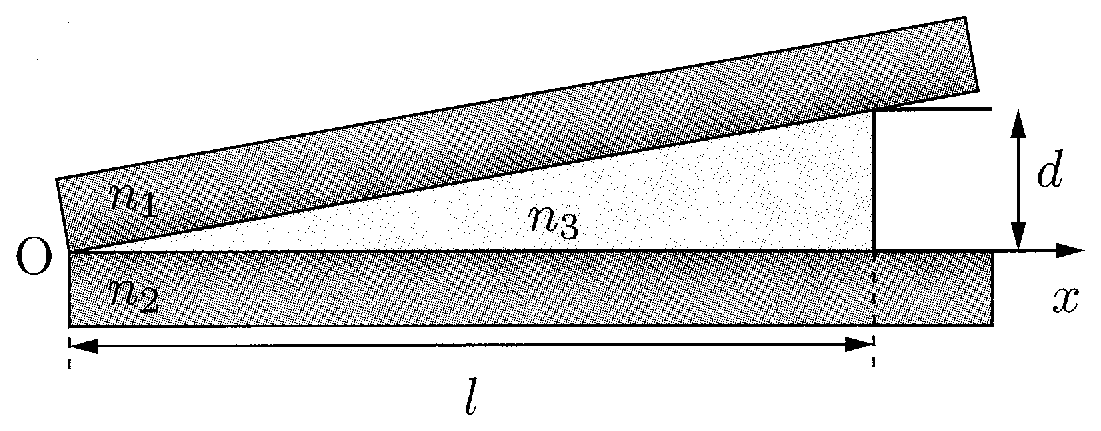
\includegraphics[keepaspectratio,width=72mm]{fig/n19_ex23.png}
\end{zuright}
\hspace{1zw}$d\ll l$であるとし，接点$\mathrm{O}$から図のように$x$軸を取る．3つの屈折率の間に$n_1<n_3<n_2$の関係がある場合について，以下の問に答えよ．
\begin{komon}
\ko{1} 位置$x\U{m}$における液体の厚み$y\U{m}$を求めよ．
\ko{2} 反射により生じる位相差を求めよ．
\ko{3} 位置$x\U{m}$において2つの反射光が強め合うための条件を整数値$m$を用いて表せ．
\ko{4} 明線が出来る位置を求めよ．
\ko{5} 隣り合う明線の間隔を求めよ．
\end{komon}
\end{reidai}

\begin{sisinE}
くさびガラスそのものだが，すき間が空気ではなく{\gtfamily 屈折率$n_3$の液体}になっている点だけが違う．ここが本問の急所で，(3)では{\gtfamily 液体中では光の速さが変化しているため，光路差を考えるときは経路差に屈折率を掛ける必要がある}．

反射による位相のずれは，{\gtfamily 上面（$n_1$と$n_3$の境界）と下面（$n_3$と$n_2$の境界）の2か所}について，それぞれ「屈折率の小さい媒質から大きい媒質へ向かう向きの反射か」を判定する．$n_1<n_3<n_2$なので2か所とも$\pi$ずれ，合計$2\pi$＝実質ずれなし，となる．ここを取り違えると明線と暗線が入れ替わってしまう．
\end{sisinE}

\Key{光路差$=$（屈折率）$\times$（経路差）．反射による位相のずれは境界の両側の屈折率の大小で決まる．}

\begin{kaitou}
\begin{komon}
\ko{1} くさびの傾き角を$\alpha$とすると，$d\ll l$より$\tan\alpha=\dfrac{d}{l}$である．よって位置$x$における液体の厚みは
       \[y=x\tan\alpha=\frac{d}{l}x\U{m}\Ans\]
\ko{2} 干渉する2つの光は，液体層の上面（屈折率$n_1$のガラスと屈折率$n_3$の液体の境界）で反射する光と，液体層の下面（屈折率$n_3$の液体と屈折率$n_2$のガラスの境界）で反射する光である．

       上面での反射は$n_1<n_3$であるから，屈折率のより大きい媒質にぶつかって反射しており，位相が$\pi$ずれる．下面での反射も$n_3<n_2$であるから同様に位相が$\pi$ずれる．よって反射による位相のずれは合計して$2\pi$であり，
       \[\text{反射により生じる位相差は}\ 0\ \text{（ずれない）}\Ans\]
\ko{3} 2つの光の経路差は液体層を往復する分の$2y\U{m}$であり，液体中を進むのでこれに屈折率$n_3$を掛けた
       \[\Delta D^\prime=n_3\times 2y=2n_3\frac{d}{l}x\]
       が光路差である．(2)より反射による位相のずれは無いので，強め合うのは光路差が真空中の波長$\lambda$の整数倍のときである．よって求める条件は，$m$を整数として
       \[2n_3\frac{d}{l}x=m\lambda\Ans\]
\ko{4} (3)を$x$について解いて，明線が出来る位置は
       \[x=m\frac{l\lambda}{2n_3d}\U{m}\quad(m=0,\,1,\,2,\,\cdots)\Ans\]
\ko{5} (4)の$m$を1つずらして差し引くことにより，
       \AnaBD{\Delta x=(m+1)\frac{l\lambda}{2n_3d}-m\frac{l\lambda}{2n_3d}=\frac{l\lambda}{2n_3d}\U{m}\Ans}
\end{komon}
\end{kaitou}

\begin{chuu}
すき間が空気（屈折率1）のときの明線間隔$\dfrac{l\lambda}{2d}$と比べると，液体で満たすと間隔が$\dfrac{1}{n_3}$倍に狭まる．これは{\gtfamily 液体中で波長が$\dfrac{\lambda}{n_3}$に縮む}ためだと考えてもよい．また本問では$\mathrm{O}$点（$x=0$）が明線になっていることに注意せよ．反射による位相のずれが合計$2\pi$（＝0）なので，接点は強め合いになる．
\end{chuu}
\end{reidaiunit}


\subsection{ニュートンリング}

\begin{zuright}{88mm}
\hspace{1zw}平面ガラスの上に大きな曲率半径$R\U{m}$をもつ平凸レンズを図のように重ね，上から単色光を当てて上からレンズを覗き込むと同心円状に明暗の環の模様ができる．この模様を{\gtfamily ニュートンリング}という．

\hspace{1zw}半径$x\U{m}$の位置（ただし$x\ll R$とする）のすき間の厚さ$d\U{m}$（図における$\mathrm{AB}$の長さ）が求まれば，くさびガラスと同様，明暗は反射による位相のずれと，経路差を波長と比較することで議論できる．
\zusep

\includegraphics[keepaspectratio,width=88mm]{text2_p12_fig1.png}
\end{zuright}

\hspace{1zw}なお，ニュートンリングでは強め合い・弱め合いとなる位置が環状になるため，それぞれ\AnaB{\gtfamily 明環，暗環}と呼ぶ．

\vspace{2mm}
\noindent{\gtfamily $\mbox{\boldmath $d$}$の求め方\MARU{1}}\\
% 近似式の変数が半径 x と衝突していたので ε に替えた（2026-09-14）。
図のように$\mathrm{H}$をとると，三平方の定理より$\mathrm{OH}=\sqrt{R^2-x^2}$なので，$|\varepsilon|\ll 1$の際に成立する$(1+\varepsilon)^{\alpha}\fallingdotseq 1+\alpha\varepsilon$の近似を用いて
\[d=\mathrm{AB}=\mathrm{O^\prime H}=R-\sqrt{R^2-x^2}=R-R\left(1-\dfrac{x^2}{R^2}\right)^{1/2}\fallingdotseq R-R\left(1-\dfrac{x^2}{2R^2}\right)=\dfrac{x^2}{2R}\]

\noindent{\gtfamily $\mbox{\boldmath $d$}$の求め方\MARU{2}}\\
図のように$\mathrm{C}$, $\mathrm{H}$をとると，$\mathrm{O^\prime C}$は円の直径なので$\angle\mathrm{CAO^\prime}=90^\circ$である．この結果を用いて角度を調べれば，二角相等で$\triangle\mathrm{AHO^\prime}\backsim\triangle\mathrm{CHA}$なので，$\mathrm{O^\prime H:AH=AH:CH}$すなわち$\mathrm{O^\prime H}=\dfrac{\mathrm{AH}^2}{\mathrm{CH}}$であり，$\mathrm{CH}=2R-d\fallingdotseq 2R$より
\[d=\mathrm{O^\prime H}=\dfrac{\mathrm{AH}^2}{\mathrm{CH}}\fallingdotseq\dfrac{x^2}{2R}\]

\noindent{\gtfamily $\mbox{\boldmath $d$}$の求め方\MARU{3}}\\
図のように$\mathrm{C}$, $\mathrm{D}$, $\mathrm{H}$をとると，$\mathrm{AH=DH}=x$, $\mathrm{O^\prime H}=d$, $\mathrm{CH}=2R-d\fallingdotseq 2R$より，方べきの定理から
\[\mathrm{AH\cdot DH=CH\cdot O^\prime H}\hspace{4mm}\therefore\ d=\mathrm{O^\prime H}=\dfrac{\mathrm{AH\cdot DH}}{\mathrm{CH}}\fallingdotseq\dfrac{x^2}{2R}\]

\begin{center}

\includegraphics[keepaspectratio,width=118mm]{text2_p12_fig2.png}
\end{center}

% 原本にはまとめ枠が無いので新設した（加筆）．
\begin{matome}{ニュートンリング}
\hspace{3mm} \MARU{1} 半径$x\U{m}$の位置のすき間の厚さ　$d\fallingdotseq\dfrac{x^2}{2R}$\hspace{4mm}（$x\ll R$）\\
\hspace{3mm} \MARU{2} 経路差　$\Delta D=2d=\dfrac{x^2}{R}$（往復分）\\
\hspace{3mm} \MARU{3} すき間が空気のときは，下側の平面ガラスでの反射だけで位相が\AnaB{$\pi$}ずれるので，\\
\hspace{3mm} 　　$\dfrac{x^2}{R}=m\lambda$（暗環　$m=0,1,2,\cdots$），$\dfrac{x^2}{R}=\left(m-\dfrac{1}{2}\right)\lambda$（明環　$m=1,2,3,\cdots$）\\
\hspace{3mm} 　　　→　{\gtfamily 中心（$m=0$の暗環）は}\AnaB{\gtfamily 暗点}\\
\hspace{3mm} \MARU{4} $x\propto\sqrt{m}$なので，環の間隔は{\gtfamily 外側にいくほど狭くなる．}
\end{matome}

%%%%% 例題24（26.2 のまとめ枠の直後）＝ 原本【例題24】〈ニュートンリング〉 %%%%%%%%%%
% 見出し(14mm)＋枠の上余白＋zuright ブロック(図59mm)が同じページに収まることを保証する。
% reidaiunit 既定の \bsNeed{30mm} だと，分割できない zuright の途中でページが尽きて
% Overfull \vbox（100pt）になり，図がページ下端をはみ出した（2026-09-14）。
\bsNeed{84mm}
\begin{reidaiunit}
\begin{reidai}{ニュートンリング}
\begin{zuright}{58mm}
\hspace{1zw}図のように，曲率半径$R\U{m}$の平凸レンズをガラス平板の上に$\mathrm{O}$点で接触するように置いた．上方から波長$\lambda\U{m}$の単色光を入射させてこの反射光を上から見ると，円形の明暗の縞模様が観測される．これについて以下の問に答えよ．
\begin{komon}
\ko{1} 接点$\mathrm{O}$から距離$r\U{m}$の点における空気層の厚さ$d\U{m}$を求めよ．ただし，$r$, $d\ll R$であることを用いて近似して答えよ．
\ko{2} 反射による位相のずれが起こる点をすべて答え，反射による位相のずれを答えよ．
% (3) も zuright の中に入れる。左の本文が図より背が低いと，残りの小問が図の
% 下端まで押し下げられて空白ができるため（2026-09-14）。
\ko{3} 中心から$m$番目の暗環の半径$r_m\U{m}$および明環の半径$r^\prime_m\U{m}$を求めよ．ただし，中心が明点もしくは暗点となる場合はそれが$m=0$に対応するようにせよ．
\end{komon}
\zusep
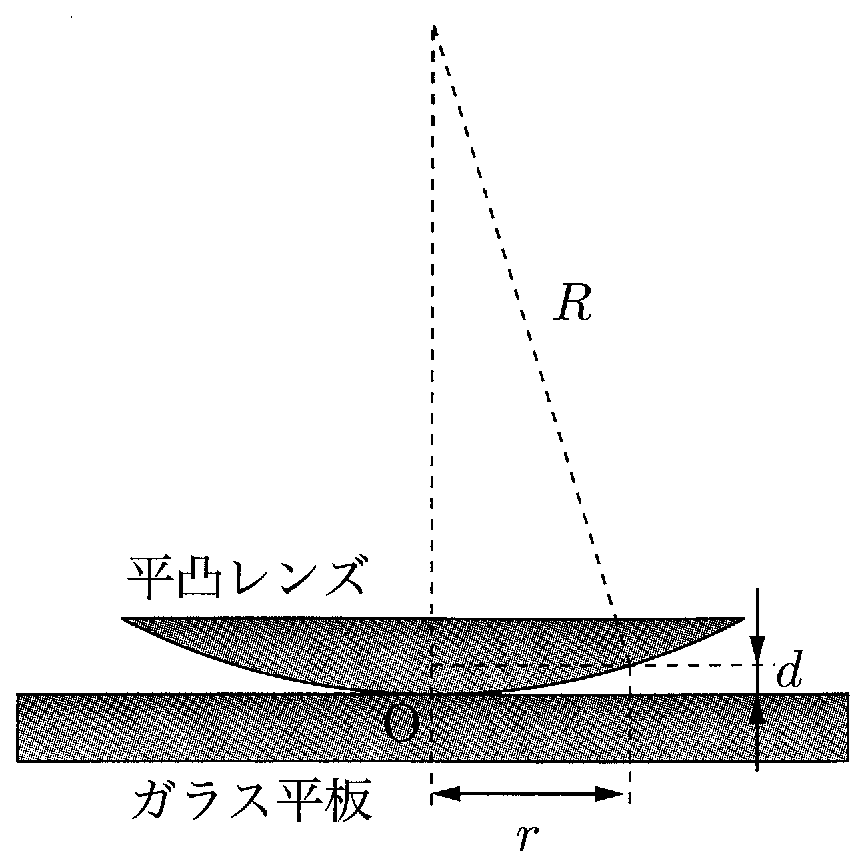
\includegraphics[keepaspectratio,width=58mm]{fig/n19_ex24.png}
\end{zuright}
\begin{komon}
\ko{4} 観測される明暗の縞模様の概形を描け．実際には明暗はぼやけるが，明線を破線で，暗線を実線で図示するだけでよい．
\end{komon}

\hspace{1zw}平凸レンズの屈折率を1.5，ガラス平板の屈折率を1.7とする．ガラス平板と平凸レンズのすき間を屈折率$n=1.6$の液体で満たした場合について以下の問に答えよ．
\begin{komon}
\ko{5} 中心は明点，暗点のいずれになるか．
\ko{6} 中心から$m$番目の暗環の半径$r_m\U{m}$および明環の半径$r^\prime_m\U{m}$を求めよ．ただし，中心が明点もしくは暗点となる場合はそれが$m=0$に対応するようにせよ．
\end{komon}
\end{reidai}

\begin{sisinE}
(1)〜(3)は本文そのままの内容である．(2)は「どこで反射するか」を1つずつ数え上げるのが要点で，{\gtfamily 平凸レンズの下面（ガラス$\to$空気）では位相はずれず，ガラス平板の上面（空気$\to$ガラス）でだけ$\pi$ずれる}．

(5)(6)が本問の山場で，{\gtfamily ガラス平板と平凸レンズのすき間における波長が$\lambda$から変化する}ことに注意する（あるいは光路差$2nd$で考える）．さらに屈折率の大小関係が$1.5<1.6<1.7$と変わるので，{\gtfamily 反射による位相のずれが2か所とも$\pi$になり，合計$2\pi$＝ずれなしになる}．その結果，明環と暗環が(3)とちょうど入れ替わる．
\end{sisinE}

\Key{ニュートンリング：$d\fallingdotseq\dfrac{r^2}{2R}$，光路差$2nd$，そして反射による位相のずれ．この3つで決まる．}

\begin{kaitou}
\begin{komon}
\ko{1} 平凸レンズの球面の中心を$\mathrm{A}$とし，接点$\mathrm{O}$から距離$r$の点の真上にある球面上の点を$\mathrm{C}$，$\mathrm{C}$から中心軸に下ろした垂線の足を$\mathrm{B}$とすると$\mathrm{AB}=R-d$である．三平方の定理より
       \[R^2=(R-d)^2+r^2\]
       これを$d$について解き，$d\ll R$として一次近似すると
       \[d=R-\sqrt{R^2-r^2}=R-R\left(1-\frac{r^2}{R^2}\right)^{\frac{1}{2}}\fallingdotseq R-R\left(1-\frac{1}{2}\frac{r^2}{R^2}\right)\]
       \[d\fallingdotseq\frac{r^2}{2R}\U{m}\Ans\]
\ko{2} 上から見た場合には，平凸レンズの下面で反射した光と，ガラス平板の上面で反射した光とが干渉する．前者は屈折率がガラス$>$空気であるから位相はずれない．後者は屈折率が空気$<$ガラスであるから位相が$\pi$ずれる．よって
       \[\text{ガラス平板の上面での反射でのみ位相がずれ，そのずれは}\ \pi\Ans\]
\ko{3} 2つの光の経路差は空気層を往復する分の$2d=\dfrac{r^2}{R}$であり，反射により位相が$\pi$ずれるので，
       \[2d=\frac{r_m^{\,2}}{R}=m\lambda\ \text{のとき弱め合い}\hspace{6mm}
         2d=\frac{r^{\prime\,2}_m}{R}=\left(m-\frac{1}{2}\right)\lambda\ \text{のとき強め合い}\]
       中心（$r=0$）は$m=0$の弱め合いに対応している．これらを解いて
       \[\left\{\begin{array}{l}\text{暗環の半径：}r_m=\sqrt{mR\lambda}\U{m}\\[2mm]\text{明環の半径：}r^\prime_m=\sqrt{\left(m-\dfrac{1}{2}\right)R\lambda}\U{m}\end{array}\right.\Ans\]
\ko{4} 中心が暗点で，暗環（実線）は$r_m=\sqrt{mR\lambda}$，明環（破線）は$r^\prime_m=\sqrt{\left(m-\frac{1}{2}\right)R\lambda}$の位置にできる．どちらも半径が$\sqrt{m}$に比例するので，外側にいくほど環の間隔は狭くなる．
       \begin{center}\AnaFig{62mm}{fig/n19_ex24_ans.png}{fig/n19_ex24_ans_blank.png}\end{center}
\ko{5} すき間の液体の屈折率$n=1.6$は，平凸レンズの屈折率1.5より大きく，ガラス平板の屈折率1.7より小さい．したがって，平凸レンズの下面での反射は$1.5<1.6$より位相が$\pi$ずれ，ガラス平板の上面での反射も$1.6<1.7$より位相が$\pi$ずれる．合計$2\pi$のずれ，すなわち{\gtfamily 反射によっては位相はずれない}．

       中心では$d=0$なので光路差も0であり，2つの光は強め合う．よって
       \[\text{中心は明点になる}\Ans\]
\ko{6} 液体中を往復するので，光路差は$2nd=\dfrac{nr^2}{R}$である．(5)より反射による位相のずれが無いので，
       \[\frac{nr^{\prime\,2}_m}{R}=m\lambda\ \text{のとき強め合い}\hspace{6mm}
         \frac{nr_m^{\,2}}{R}=\left(m-\frac{1}{2}\right)\lambda\ \text{のとき弱め合い}\]
       中心（$r=0$）は$m=0$の強め合いに対応している．$n=1.6$を代入してこれらを解くと
       \AnaBD{\left\{\begin{array}{l}\text{暗環の半径：}r_m=\sqrt{\dfrac{\left(m-\frac{1}{2}\right)R\lambda}{1.6}}=\dfrac{1}{4}\sqrt{10\left(m-\dfrac{1}{2}\right)R\lambda}\U{m}\\[3mm]\text{明環の半径：}r^\prime_m=\sqrt{\dfrac{mR\lambda}{1.6}}=\dfrac{1}{4}\sqrt{10mR\lambda}\U{m}\end{array}\right.\Ans}
\end{komon}
\end{kaitou}

\begin{chuu}
(3)と(6)で明環と暗環がちょうど入れ替わっている．これは{\gtfamily 反射による位相のずれが$\pi$から$0$へ変わった}ためである．ニュートンリングの問題では，すき間を何で満たすか，上のレンズと下の板の屈折率がいくつかによって毎回この判定が変わるので，公式として暗記せず必ずその都度考えること．
\end{chuu}
\end{reidaiunit}


\subsection{平行薄膜による干渉}

\begin{zuright}{78mm}
\hspace{1zw}シャボン玉のようなごく薄い平行薄膜層が空気に挟まれており，この厚さ$d\U{m}$の薄膜層（屈折率を$n$とする）に図のような角度$i$で入射してくる真空中での波長が$\lambda\U{m}$の光波について考える．簡単のため，空気の屈折率を1とする．

\hspace{1zw}図の$\mathrm{A_1\to B_1}$へ入射してきた光波の一部分は反射され，残りは図のように屈折角$r$で薄膜層に入る．$\mathrm{D}$点に達した光の一部は空気層へ出るが，残りは反射されて図の$\mathrm{C_2}$点へ向かい，$\mathrm{C_2}$点でも同様に一部は$\mathrm{Q}$の方向へ屈折して出ていき，一部は層内部へ反射される．
\zusep
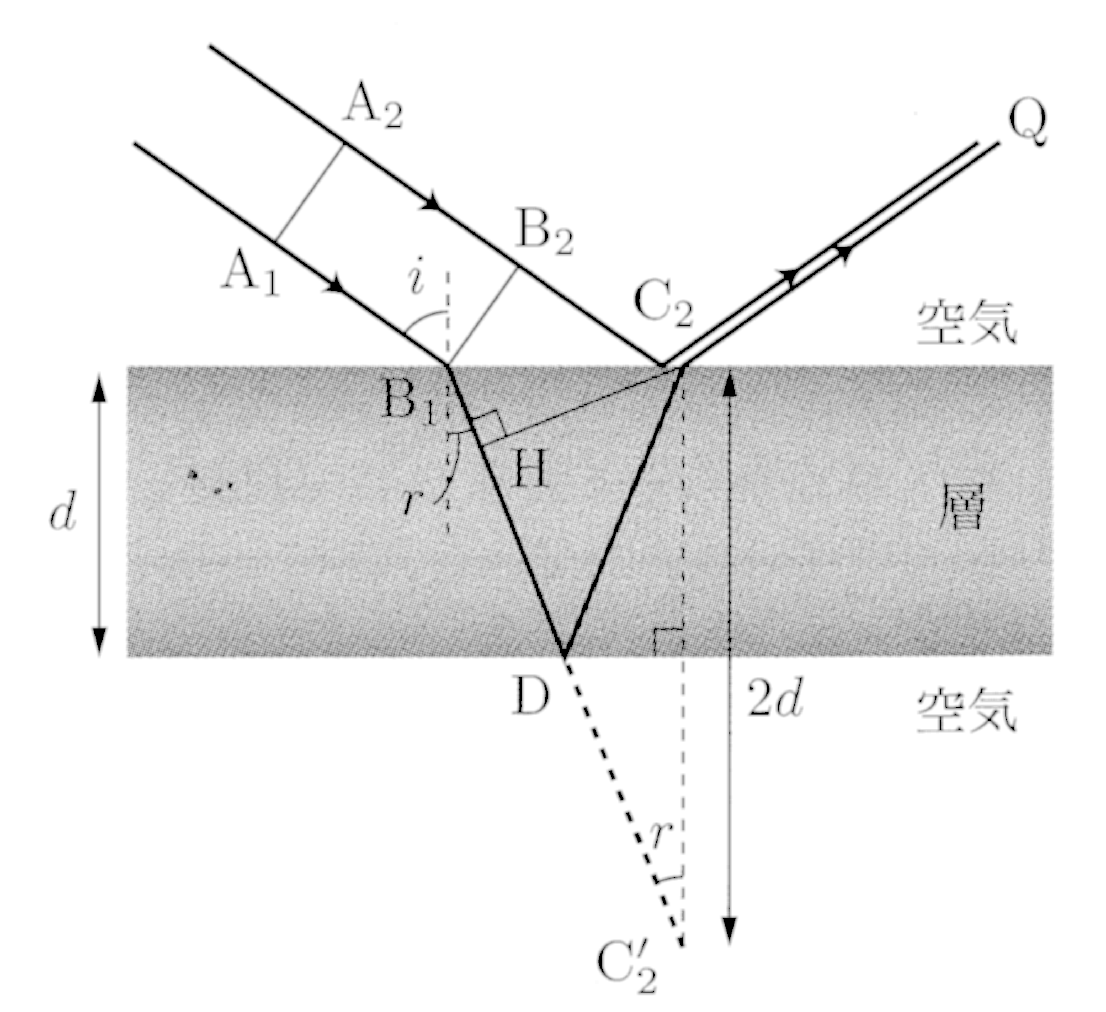
\includegraphics[keepaspectratio,width=78mm]{fig/n19_thinfilm.png}
\end{zuright}

\hspace{1zw}反射されてくる光を$\overrightarrow{\mathrm{QC_2}}$の方向から観測する場合，上で述べたような経路をたどってくる光と，$\mathrm{A_2\to B_2\to C_2\to Q}$というように直接$\mathrm{C_2}$点で反射する光とが重なって観測される．この2つの光の干渉について考える．

\hspace{1zw}層内部でのこの光波の波長は$\lambda^\prime=\AnaB{$\dfrac{\lambda}{n}$}\U{m}$となる．まず，経路差によりどれだけの位相のずれが生じるのかを考えてみよう．

\hspace{1zw}入射してくる光は平行波なので進行方向に垂直な面が波面となる．ゆえに$(\mathrm{A_1},\mathrm{A_2})$および$(\mathrm{B_1},\mathrm{B_2})$は同一波面上にあり，常に位相が一致している．よって，経路差は$\mathrm{B_1\to D\to C_2}$と$\mathrm{B_2\to C_2}$の差である．しかし空気中と層内部とでは光波の波長が異なるため，単純に距離の差をとって$\lambda\U{m}$で割ったのでは正しく何波長分ずれるかが計算できない．そのため，光路長の差として
\[n\left(\overline{\mathrm{B_1D}}+\overline{\mathrm{DC_2}}\right)-\overline{\mathrm{B_2C_2}}\]
を計算し，この長さと真空中の波長$\lambda\U{m}$を比較することになる．

\hspace{1zw}さらに，ホイヘンスの原理を用いると，光路差による位相のずれをより簡単にまとめることができる．$\mathrm{C_2}$から直線$\mathrm{B_1D}$に下ろした垂線の足の点を$\mathrm{H}$とすると，ホイヘンスの原理より$\mathrm{C_2}$点と$\mathrm{H}$点は同一波面上にある（屈折の法則参照）．よって，光路差による位相のずれは$\mathrm{H\to D\to C_2}$の部分によるずれのみを考えればよい．さらに，$\mathrm{C_2}$点を下側の境界面に対称に折り返した点を$\mathrm{C_2^\prime}$とすると，
\[\mathrm{HD+DC_2=HD+DC_2^\prime=HC_2^\prime}=2d\cos r\]
となり，この幾何学的距離を光路長に換算することにより，
\[\text{光路差}\hspace{4mm}\Delta D^\prime=2nd\cos r\]
と簡単に求められる．

% 原本（第26回 26.3）は「まず，経路差により…」と書き出しながら，反射による位相の
% ずれを最後まで扱わずに節が終わっていた。直後の例題25(1)がまさにそこを問うので，
% 本文とまとめ枠に補った（2026-09-14 加筆）。
\hspace{1zw}次に，反射による位相のずれを考えよう．くさびガラス・ニュートンリングと同じく，{\gtfamily 反射が起こるのは2か所}である．シャボン玉のように層の上下がともに空気（屈折率1）で，層の屈折率が$n>1$の場合は，

\begin{description}
\item[$\mathrm{C_2}$点（上側の境界面）] 空気（1）から層（$n$）へ向かう，すなわち屈折率のより大きい媒質にぶつかる反射なので，位相が$\pi$ずれる．
\item[$\mathrm{D}$点（下側の境界面）] 層（$n$）から空気（1）へ向かう，すなわち屈折率のより小さい媒質にぶつかる反射なので，位相は\AnaB{ずれない}．
\end{description}

\noindent となり，反射により合計して位相が$\pi$ずれる．したがって$\overrightarrow{\mathrm{C_2Q}}$方向へ出ていく光については，

\[2nd\cos r=\left(m-\dfrac{1}{2}\right)\lambda\ \text{のとき強め合い}\hspace{6mm}2nd\cos r=m\lambda\ \text{のとき弱め合い}\]

\hspace{1zw}ただし，この$\pi$は「上下がともに空気」の場合の値にすぎない．層の下が水や別のガラスであれば下側の反射でも$\pi$ずれて合計$2\pi$（＝ずれなし）になり，強め合いと弱め合いが入れ替わる．{\gtfamily 光路差$2nd\cos r$は形が変わらないが，反射による位相のずれは問題ごとに2か所を数え直さねばならない．}

\begin{matome}{平行薄膜による干渉}
\hspace{3mm} \MARU{1} 2つの経路の光路差　$\Delta D^\prime=2nd\cos r$\\
\hspace{3mm} 　　（$r$は{\gtfamily 屈折角}．入射角$i$で書くなら$\Delta D^\prime=\AnaB{$2d\sqrt{n^2-\sin^2 i}$}$）\\
\hspace{3mm} \MARU{2} 反射による位相のずれは{\gtfamily 上下2か所}を数える．上下がともに空気なら合計$\pi$\\
\hspace{3mm} 　　→　$2nd\cos r=\left(m-\dfrac{1}{2}\right)\lambda$（強め合い），$2nd\cos r=m\lambda$（弱め合い）
\end{matome}

%%%%% 例題25（26.3 のまとめ枠の直後）＝ 原本【例題25】〈平行薄膜による干渉〉 %%%%%%%%%%
\begin{reidaiunit}
\begin{reidai}{平行薄膜による干渉}
\begin{zuright}{56mm}
\hspace{1zw}水面\hspace{0.1zw}III\hspace{0.1zw}の上に一様な厚さ$d\U{m}$，屈折率$n$の油\hspace{0.1zw}II\hspace{0.1zw}の薄膜が乗っている．これに波長$\lambda\U{m}$の単色光を，屈折率1の大気\hspace{0.1zw}I\hspace{0.1zw}から薄膜へ入射させると屈折角$r$で屈折した．これについて以下の問に答えよ．
% 小問は zuright の中に入れる（外に出すと図の下端まで押し下げられて空白ができる）。
\begin{komon}
\ko{1} $\mathrm{D}$点で観測される図の2つの経路から来る波について，反射による位相のずれはどれだけか．ただし，この油\hspace{0.1zw}II\hspace{0.1zw}の屈折率$n$は水\hspace{0.1zw}III\hspace{0.1zw}の屈折率よりも小さいものとする．
\ko{2} $\mathrm{C}$点で直接反射されて$\mathrm{D}$点に来る光と，$\mathrm{A}$点から$\mathrm{B}$点を回って$\mathrm{D}$点に来る光との光路差を求めよ．
\ko{3} $\mathrm{C}$点から来る光を$\mathrm{D}$点で観測したとき，暗くなるための条件式を示せ．
\end{komon}
\zusep
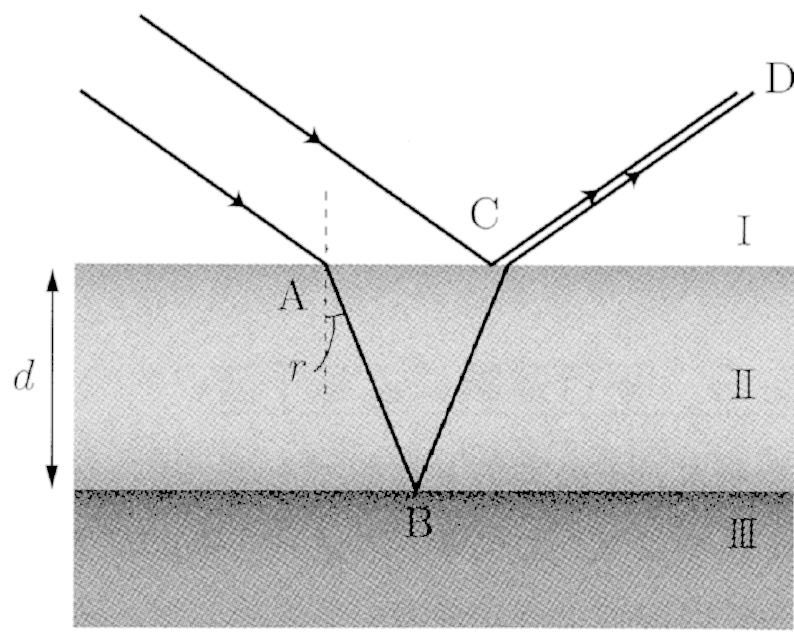
\includegraphics[keepaspectratio,width=56mm]{fig/n19_ex25.png}
\end{zuright}
% (4) は 2026-09-14 にユーザー指示で新設。原本には無い設問。
% 現実の油（n≒1.5）は水（n≒1.33）より屈折率が大きく，直後の練習[58]もその設定
% （油1.5／水1.3）なので，(1)〜(3) の裏返しを例題のうちに確認させる。
\begin{komon}
\ko{4} 実際の油は水よりも屈折率が大きいことが多い．油\hspace{0.1zw}II\hspace{0.1zw}の屈折率$n$が水\hspace{0.1zw}III\hspace{0.1zw}の屈折率よりも大きい場合，(3)の答えはどうなるか．
\end{komon}
\end{reidai}

\begin{sisinE}
% 旧版の指針は「C点から油膜の上面に下ろした垂線」「B点を折り返す」と書いていたが，
% C は上面上の点・B は下側境界面上の点なので，どちらも取り違え（2026-09-14 訂正）。
本文の内容をそのまま使う問題である．(2)の光路差$2nd\cos r$は，{\gtfamily $\mathrm{C}$点と，$\mathrm{C}$点から屈折光線$\mathrm{AB}$に下ろした垂線の足とが同一波面上にある}ことと，{\gtfamily $\mathrm{C}$点を下側の境界面（油と水の境界）に対称に折り返す}ことの2つで導ける．説明の仕方まで含めて覚えておくこと．また屈折率$n$を掛け忘れないように注意．

(1)は2か所の反射（$\mathrm{C}$点＝大気と油の境界，$\mathrm{B}$点＝油と水の境界）をそれぞれ判定する．$1<n$かつ$n<$（水の屈折率）なので{\gtfamily 2か所とも$\pi$ずれ，合計$2\pi$＝実質ずれなし}となる．したがって(3)の「暗くなる条件」は光路差が半波長の奇数倍，である．

(4)は$\mathrm{B}$点での大小関係だけがひっくり返る．{\gtfamily 反射による位相のずれは$\mathrm{C}$点の$\pi$だけ}になるので，強め合いと弱め合いが(3)と入れ替わる．光路差の式$2nd\cos r$は何も変わらないことを確認せよ．
\end{sisinE}

\Key{2つの経路の光路差　$\Delta D^\prime=2nd\cos r$}

\begin{kaitou}
\begin{komon}
\ko{1} 反射が起こるのは，$\mathrm{C}$点（大気\hspace{0.1zw}I\hspace{0.1zw}と油\hspace{0.1zw}II\hspace{0.1zw}の境界）と$\mathrm{B}$点（油\hspace{0.1zw}II\hspace{0.1zw}と水\hspace{0.1zw}III\hspace{0.1zw}の境界）の2か所である．

       $\mathrm{C}$点では大気の屈折率$1<n$であるから，屈折率のより大きい媒質にぶつかって反射しており位相が$\pi$ずれる．$\mathrm{B}$点でも$n<$（水の屈折率）であるから同様に位相が$\pi$ずれる．よって合計$2\pi$となり，
       \[\text{反射による位相のずれは}\ 0\ \text{（ずれない）}\Ans\]
\ko{2} $\mathrm{C}$点から直線$\mathrm{AB}$に下ろした垂線の足を$\mathrm{C^\prime}$とすると，ホイヘンスの原理より$\mathrm{C}$点と$\mathrm{C^\prime}$点は同一波面上にある．よって経路差を生むのは$\mathrm{C^\prime\to B\to C}$の部分だけである．

       さらに$\mathrm{C}$点を油と水の境界面に対称に折り返した点を$\mathrm{C^{\prime\prime}}$とすると，
       \[\mathrm{C^\prime B+BC=C^\prime B+BC^{\prime\prime}=C^\prime C^{\prime\prime}}=2d\cos r\]
       である．この部分は屈折率$n$の油の中なので，光路差は
       \[\Delta D^\prime=2nd\cos r\U{m}\Ans\]
\ko{3} (1)より反射による位相のずれは無いので，弱め合って暗くなるのは光路差が真空中の半波長の奇数倍になるときである．よって，$m$を整数として
       \AnaBD{2nd\cos r=\left(m-\frac{1}{2}\right)\lambda\Ans}
\ko{4} $\mathrm{C}$点での反射は大気の屈折率$1<n$のままなので位相が$\pi$ずれる．一方$\mathrm{B}$点での反射は$n>$（水の屈折率）となり，屈折率のより小さい媒質にぶつかって反射することになるので，位相はずれない．よって反射による位相のずれは合計$\pi$である．

       (2)の光路差$\Delta D^\prime=2nd\cos r\U{m}$そのものは変わらない．反射で$\pi$ずれるので，暗くなる（弱め合う）のは光路差が真空中の波長の整数倍のときであり，
       \[2nd\cos r=m\lambda\Ans\]
       すなわち(3)の条件式で強め合いと弱め合いが入れ替わる．
\end{komon}
\end{kaitou}

\end{reidaiunit}


\newpage

% 練習番号：第14〜18回の練習題数の合計は 10+10+8+14+11＝53題．よって第19回は［54］から．
\setcounter{qno}{53}

\filbreak
\Rank{A問題}

\Mon{基本公式の確認}

\hspace{1zw}空気の絶対屈折率を1として，以下の設問に答えよ．
\begin{komon}
\ko{1} 真空中での波長が$\lambda\U{m}$の単色光を，水の上に作った薄い有機溶媒の膜に対して垂直に入射させる．この有機溶媒の絶対屈折率は水の絶対屈折率よりも大きく，これを$n$とするとき，反射光が明るくなる最小の膜厚はいくらか．
\ko{2} 間の層が空気である微小頂角$\theta\U{rad}$のくさびガラスに対して，上面から垂直に波長$\lambda\U{m}$の平行光線を入射させた．このとき，くさびガラスを上面から見たときに見える干渉縞の明線間隔はいくらか．ただし$\theta$が1より十分小さい場合は，$\sin\theta\fallingdotseq\tan\theta\fallingdotseq\theta$, $\cos\theta\fallingdotseq 1$の近似を用いよ．
\end{komon}

\filbreak
\Rank{B問題}

\Mon{光学的距離（ジャマンの実験）}

\begin{zuright}{70mm}
\hspace{1zw}右図のように，スリット$\mathrm{P}$から出た波長$\lambda=5.90\times 10^{-7}\U{m}$の単色光を，レンズ$\mathrm{L_1}$を用いて平行光として，複スリット$\mathrm{S_1}$, $\mathrm{S_2}$に入射させる．スリット$\mathrm{S_1}$, $\mathrm{S_2}$の先に進んだ光は，両端にガラス窓を持つ長さ$l=1.00\times 10^{-1}\U{m}$の同一の管$\mathrm{T_1}$, $\mathrm{T_2}$を通過したのち，再びレンズ$\mathrm{L_2}$によってスクリーン上の一点$\mathrm{Q}$に集光される．
\zusep
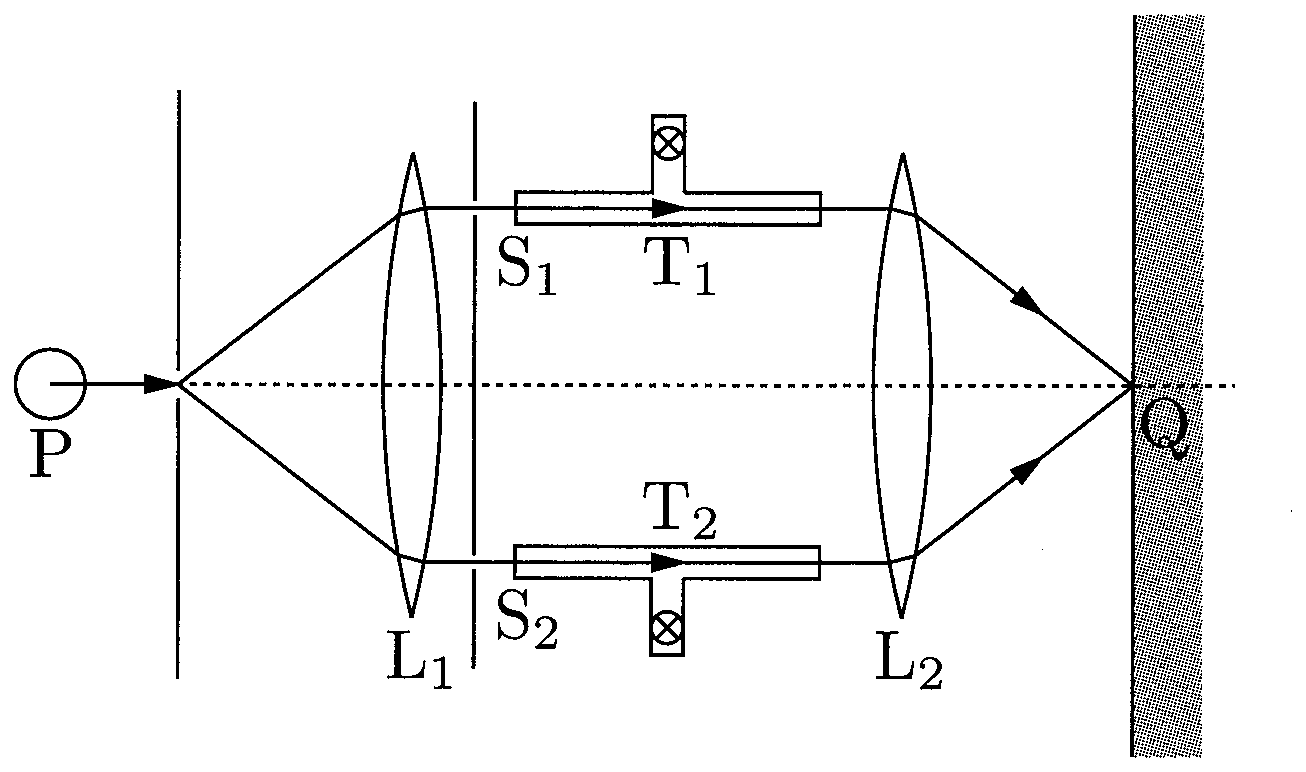
\includegraphics[keepaspectratio,width=70mm]{fig/n19_p55_jamin.png}
\end{zuright}

\hspace{1zw}今，管$\mathrm{T_1}$, $\mathrm{T_2}$を両方とも真空にしておき，$\mathrm{Q}$点にやってくる二つの光の干渉を観察すると，$\mathrm{P}$, $\mathrm{L_1}$, $\mathrm{L_2}$, $\mathrm{Q}$および複スリット$\mathrm{S_1}$, $\mathrm{S_2}$の中心が同一軸上にあるため，光路差なく二つの光が干渉し，$\mathrm{Q}$点で二つの光が強め合って明るくなった．この状態から，管$\mathrm{T_2}$のみに，ある気体を少しずつ入れていったところ，$\mathrm{Q}$点では暗くなったり明るくなったりすることが交互に観察された．その回数は管$\mathrm{T_2}$内の気体の圧力に比例し，圧力が$1.00\times 10^5\U{Pa}$になった際にちょうど50回目（ただし初めの状態を0回目とする）の明るい状態となった．これについて，以下の設問に答えよ．
\begin{komon}
\ko{1} 管$\mathrm{T_2}$に入れた気体の圧力が$p\times 10^5\U{Pa}$になったときのこの気体の絶対屈折率を$n$とする．このとき，$\mathrm{Q}$点にやってくる二つの光の光路差を，$n$, $l$を用いて表せ．
\ko{2} $\mathrm{Q}$点で光が強め合うときの管$\mathrm{T_2}$内の気体の絶対屈折率を，整数値$m$および$\lambda$, $l$を用いて表せ．
\ko{3} 圧力が$1.00\times 10^5\U{Pa}$のときのこの気体の絶対屈折率はいくらか．
\ko{4} この気体の絶対屈折率$n$と，圧力$p\times 10^5\U{Pa}$の関係式を求めよ．
\end{komon}

\Mon{くさびガラスの干渉}

\begin{zuright}{74mm}
\hspace{1zw}空気中で，平面ガラス$\mathrm{G_1}$の上に平面ガラス$\mathrm{G_2}$をのせ，一端に薄い紙$\mathrm{P}$を挟んで，$\mathrm{G_1}$の面に垂直に波長$\lambda\U{m}$の単色光を当てて真上から観察したところ，$\mathrm{G_1}$と$\mathrm{G_2}$の接触している線$\mathrm{A}$に平行に明線間隔$b\U{m}$の干渉縞が見られた．

\hspace{1zw}$\mathrm{A}$側から数えて$m$番目の明線の位置の$\mathrm{A}$からの距離を$x\U{m}$，その位置の空気層の厚さを$d\U{m}$とする．また，$\mathrm{A}$から紙の先端$\mathrm{B}$までの距離を$l\U{m}$とする．この紙は非常に薄いため，光は$\mathrm{G_2}$の面に対しても垂直であるとみなしてよいものとして以下の設問に答えよ．
\zusep
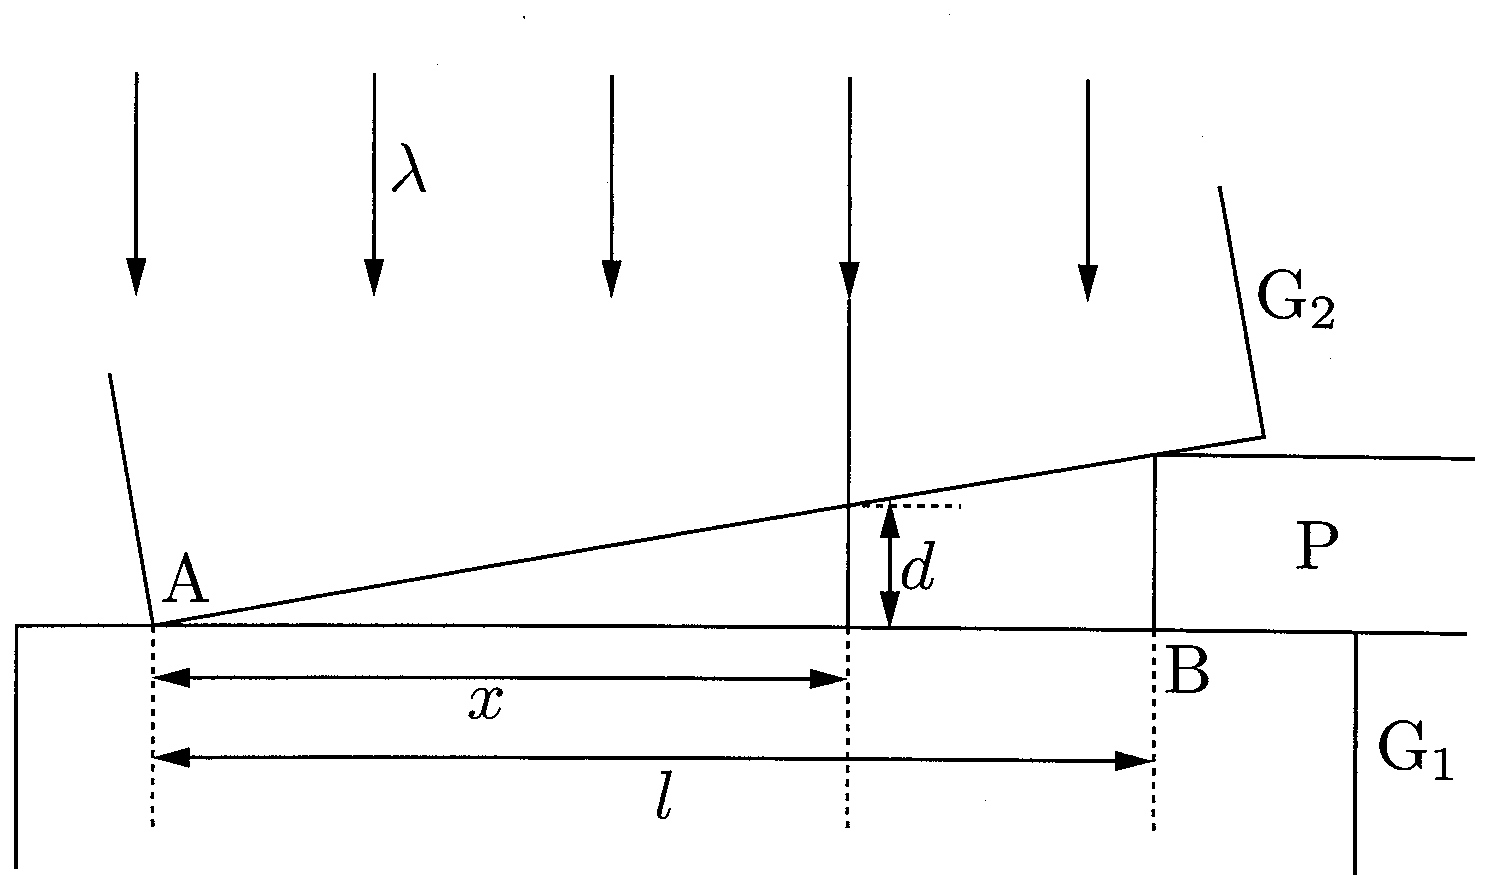
\includegraphics[keepaspectratio,width=74mm]{fig/n19_p56_wedge.png}
\end{zuright}
\begin{komon}
\ko{1} $d$を$\lambda$, $m$を用いて表せ．
\ko{2} 紙の厚さを，$\lambda$, $l$, $b$を用いて表せ．
% 原本は λ=6.0×10^{-10}[m]（解答も紙の厚さ 1.2×10^{-8}[m]）だが，これはX線の波長域で，
% 「単色光を当てて真上から観察し，暗線を41本数える」という設定と両立しない．
% 紙の厚さ 12nm も非現実的なので，可視光 6.0×10^{-7}[m] の誤植と判断して直した．
% これに伴い解答の紙の厚さも 1.2×10^{-5}[m]＝12μm になる（2026-09-05 ユーザー判断）。
\ko{3} $\lambda=6.0\times 10^{-7}\U{m}$のとき，$\mathrm{B}$の位置も暗線で，$\mathrm{A}$と$\mathrm{B}$を含めて41本の暗線が見られた．紙の厚さを（数値で）求めよ．
\ko{4} $\mathrm{G_1}$と$\mathrm{G_2}$の間に透明な液体を満たしたら，縞の間隔が$b^\prime\U{m}$になった．この液体の屈折率を$b$, $b^\prime$を用いて表せ．
\end{komon}

\Mon[\Sitei]{ニュートンリング}

\begin{zuright}{56mm}
\hspace{1zw}図のように，曲率半径$R\U{m}$の平凸レンズをガラス平板の上に$\mathrm{O}$点で接触するように置いた．上方から波長$\lambda\U{m}$の単色光を入射させてこの反射光を上から見ると，円形の明暗の縞模様（ニュートンリング）が観測される．これについて以下の設問に答えよ．
\begin{komon}
\ko{1} 接点$\mathrm{O}$から距離$r\U{m}$の点における空気層の厚さ$d$を求めよ．ただし，$r$, $d\ll R$であることを用いて近似して答えよ．
\ko{2} 中心から$m$番目の暗環の半径$r_m$および明環の半径$r^\prime_m$を求めよ．ただし，中心が明点もしくは暗点となる場合はそれが$m=0$に対応するようにせよ．
\end{komon}
\zusep
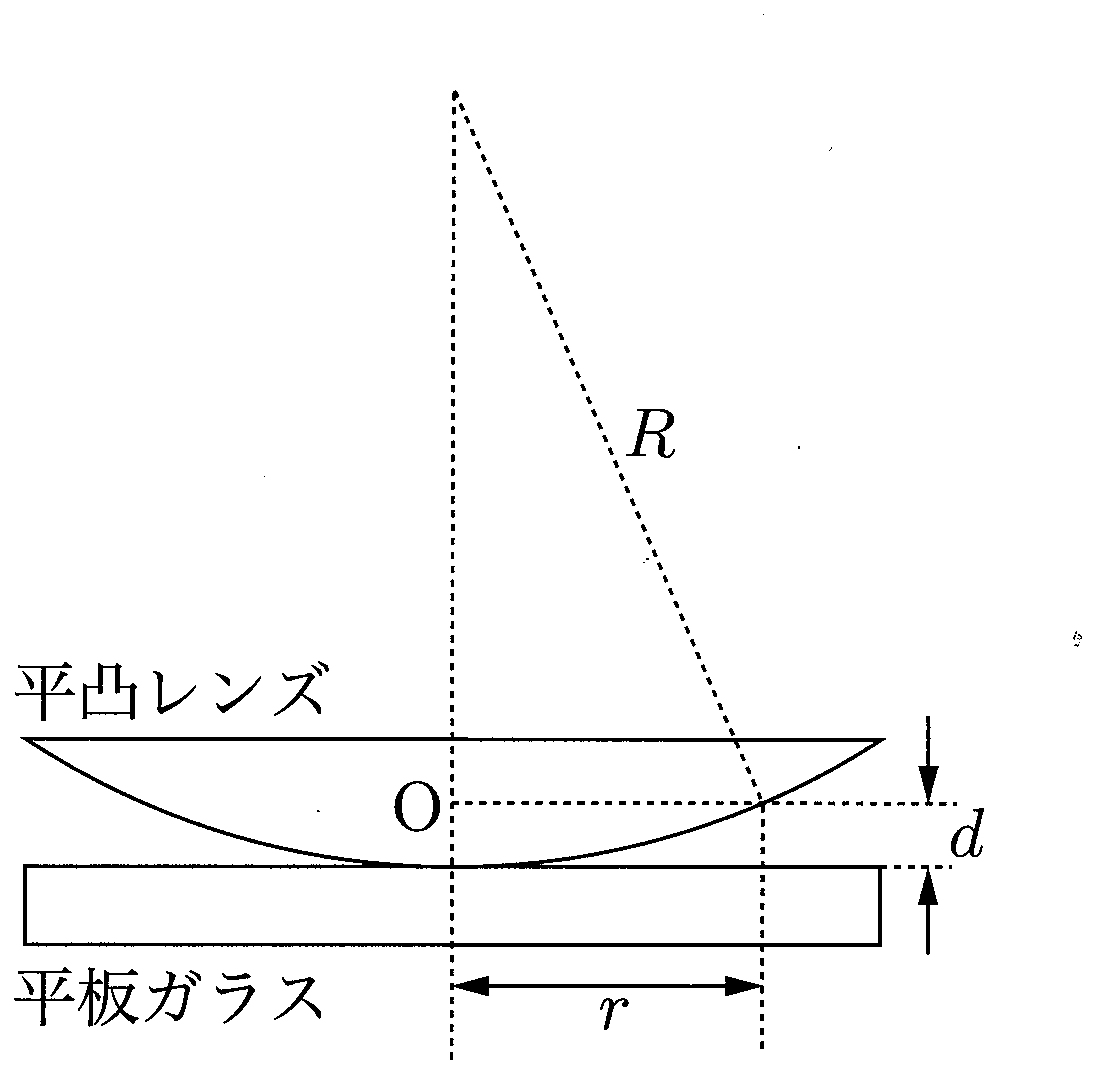
\includegraphics[keepaspectratio,width=56mm]{fig/n19_p57_newton.png}
\end{zuright}
\begin{komon}
\ko{3} 明環・暗環の間隔は，外側にいくほど狭くなるか，広くなるか．理由をつけて答えよ．
\ko{4} $\lambda=5.5\times 10^{-7}\U{m}$のとき，中心から数えて8番目の明環が半径$5.0\times 10^{-3}\U{m}$のところに観測された．この位置のすき間の間隔はいくらか．また，レンズの曲率半径はいくらか．
\ko{5} この平凸レンズを上方向に平行にゆっくりと持ち上げていくと，観察されるニュートンリングはどのように変化するか．リングの動く向き，および中心付近のリングの様子（リングが消失もしくは生成するか，もしくは全体が拡大・縮小するか）を答えよ．
\ko{6} (5)の操作によって，リングがちょうど5本分だけずれた．平凸レンズを持ち上げた距離はどれだけか．$\lambda$を用いて答えよ．
% 原本は「この反射光を下面から観察する」．解答では「リングを直接通り抜けていく光と，
% 空気層の部分を往復してから下へ抜ける光」の干渉として扱っている（＝透過光の観察）．
\ko{7} 再び平凸レンズをガラス平板に接触させる．上方から波長$\lambda\U{m}$の単色光を入射させてこの光を下面から観察する場合の，中心から$m$番目の暗環の半径$r_m$および明環の半径$r^\prime_m$を求めよ．ただし，中心が明点もしくは暗点となる場合はそれが$m=0$に対応するようにせよ．
\end{komon}

\Mon[\Sitei]{平行薄膜による干渉}

\begin{zuright}{58mm}
\hspace{1zw}絶対屈折率$n_0=1.3$の水面の上に，絶対屈折率$n=1.5$，厚さ$d\U{m}$の薄い平行な油膜が浮いており，これに対して波長$\lambda\U{m}$の平行光線を入射角$i$で照射した．この平行薄膜による反射光を$\mathrm{E}$の方向で観察し，図の$\mathrm{ABCE}$の経路で来る光と，$\mathrm{C}$点で直接反射してくる光の二つの光の干渉を考える場合について，以下の設問に答えよ．ただし，空気の絶対屈折率を1とする．
\zusep
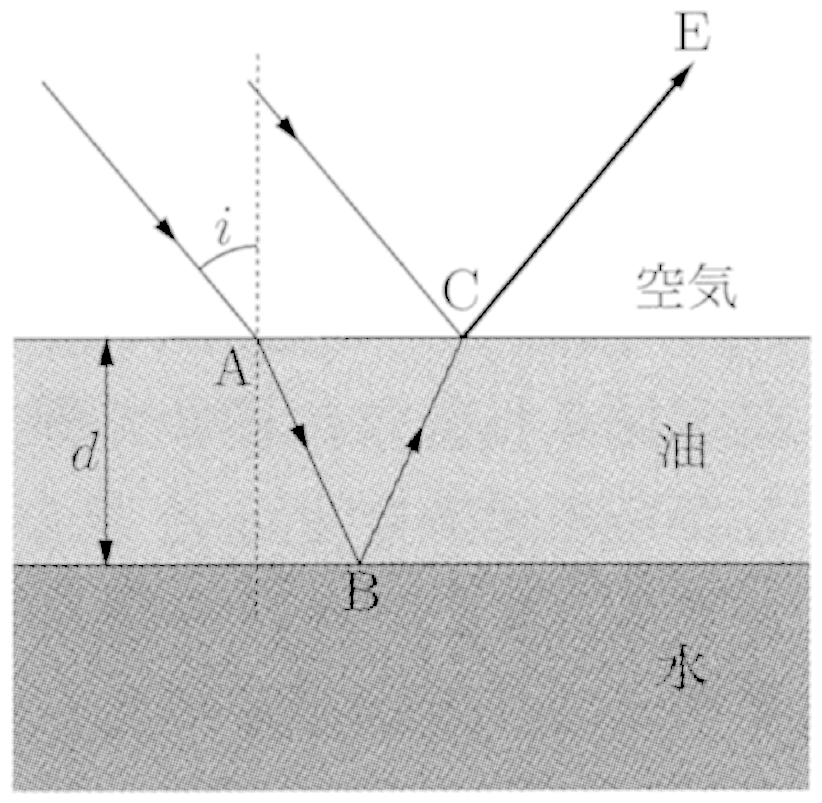
\includegraphics[keepaspectratio,width=58mm]{fig/n19_p58_oil.png}
\end{zuright}
\begin{komon}
\ko{1} この二つの光の光路差を$n$, $d$, $i$を用いて表せ．
\ko{2} このとき強め合う波長を，整数値$m$および$d$, $n$, $i$を用いて表せ．
\ko{3} この油膜（$d=5.0\times 10^{-4}\U{mm}$とする）に対して，垂直に白色光（可視光領域である$380\U{nm}$〜$780\U{nm}$のすべての波長を含む光）を照射したとき，強め合う反射光の波長を求めよ．
% (3)は mm，(4)は m で書かれており，2000倍の変更なのに単位が違って誤読しやすい。
% mm と m を併記した（2026-09-14）。
\ko{4} (3)において，もし油膜の厚さが$d=1.0\U{mm}=1.0\times 10^{-3}\U{m}$であったとすると，反射光は何色に見えるか．
\end{komon}

\filbreak
\Rank{C問題}

\Mon{ゆがみのあるくさびガラス}

\begin{zuright}{66mm}
\hspace{1zw}図1のように平板ガラス$\mathrm{A}$, $\mathrm{B}$を微小角$\theta$だけ傾けて配置し，$\mathrm{A}$の上方から$\mathrm{B}$に対して垂直に波長$\lambda\U{m}$の平行光線を入射し，これを$\mathrm{A}$の上面から観察すると，等間隔の平行な縞模様が観察される．これについて以下の設問に答えよ．ただし，微小角$|\theta|\ll 1$に対して成立する近似式$\sin\theta\fallingdotseq\tan\theta\fallingdotseq\theta$, $\cos\theta\fallingdotseq 1$を利用せよ．
\zusep
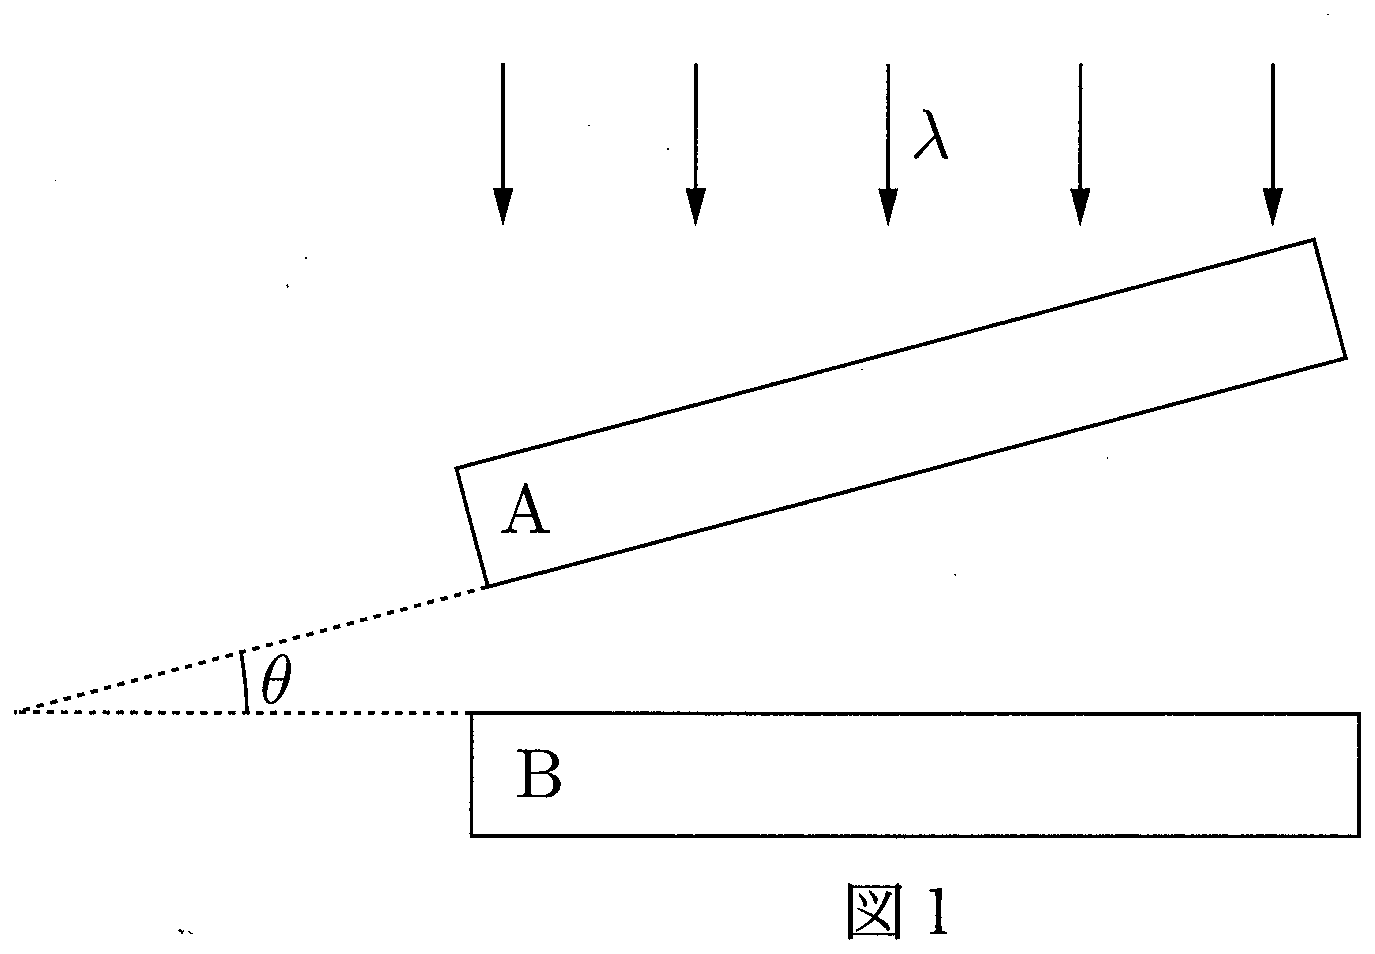
\includegraphics[keepaspectratio,width=66mm]{fig/n19_p59_zu1.png}
\end{zuright}
\begin{komon}
\ko{1} 隣り合う暗線の間隔$d$を$\lambda$, $\theta$を用いて表せ．
\ko{2} ガラス$\mathrm{A}$を上方または下方に平行移動させたところ，干渉縞全体が，図1の右方向に縞模様ちょうど10本分だけずれた．$\mathrm{A}$板を上方，下方いずれにどれだけの距離だけ動かしたかを答えよ．
\ko{3} 干渉縞をよく観察したところ，図2のように曲がっている部分があり，暗線のずれは最大2本分であった．$\mathrm{B}$の板の上面が完全な平面になっているとすると，$\mathrm{A}$板の下面はふくらんでいるか，それともへこんでいるか．またその最大のふくらみまたはへこみはどれだけかを求めよ．
       \begin{center}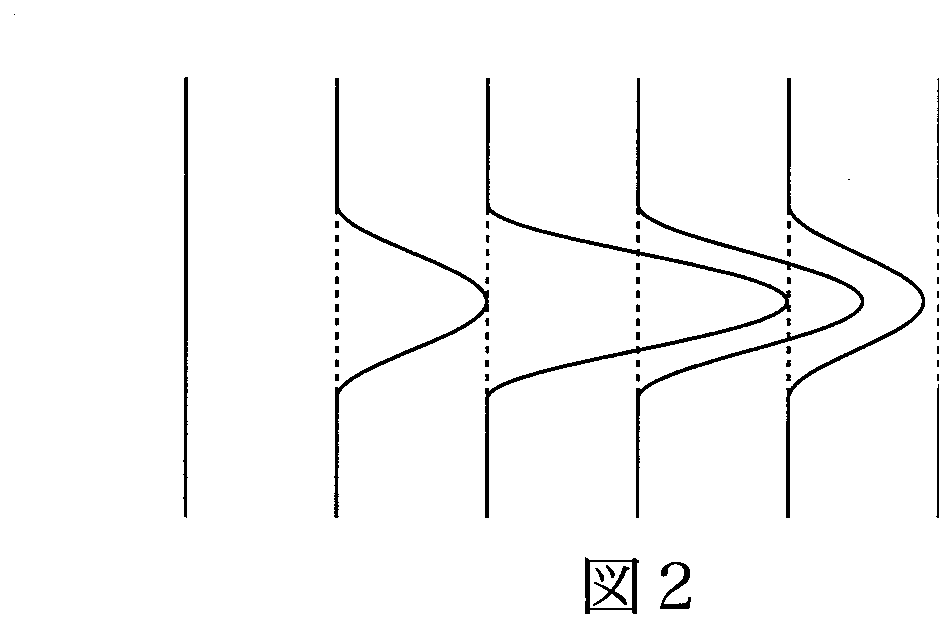
\includegraphics[keepaspectratio,width=52mm]{fig/n19_p59_zu2.png}\end{center}
\end{komon}

\Mon{円形スリットによる干渉}

\begin{zuright}{46mm}
\hspace{1zw}不透明な平板に，図1のような点$\mathrm{O}$を中心とする小穴$\mathrm{S_0}$と同心円の狭いスリット$\mathrm{S_1}$, $\mathrm{S_2}$, $\cdots$, $\mathrm{S}_m$, $\cdots$, $\mathrm{S}_N$が刻まれている（$N$は100程度の値である）．スリット$\mathrm{S}_m$の半径を$r_m\U{m}$とおく．
\zusep
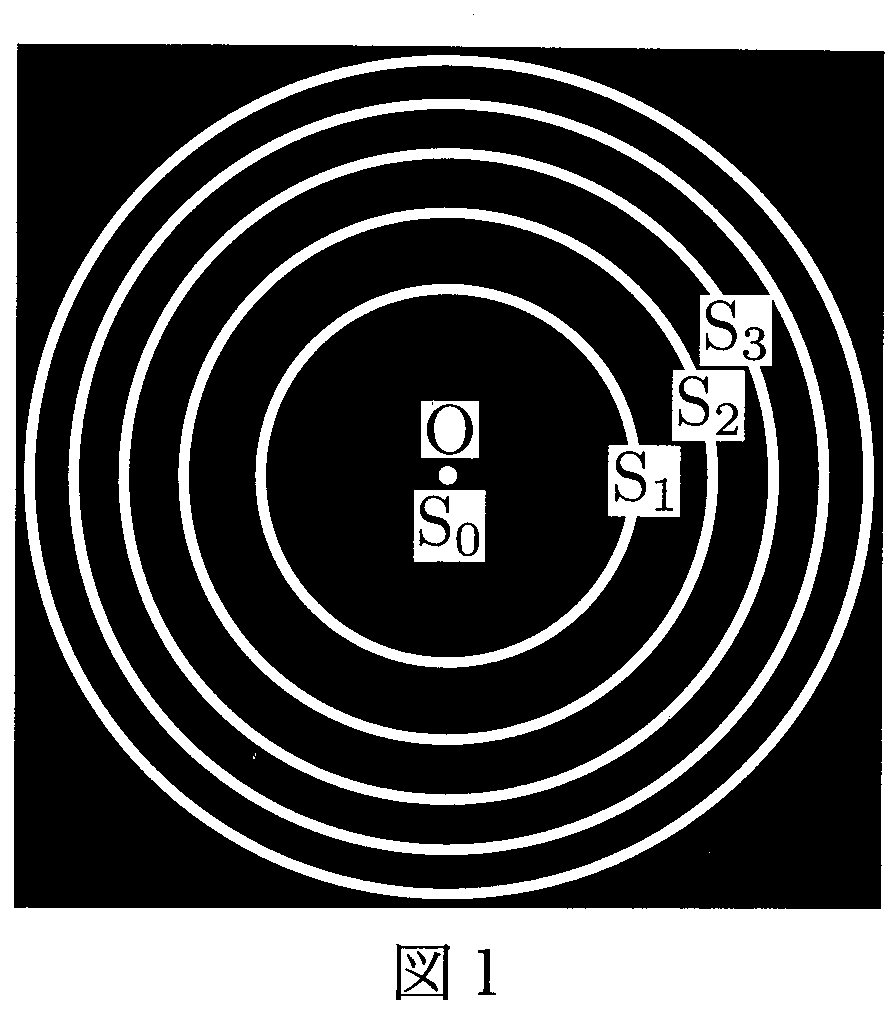
\includegraphics[keepaspectratio,width=46mm]{fig/n19_p60_zu1.png}
\end{zuright}

\begin{zuright}{58mm}
\hspace{1zw}図2のように，$\mathrm{O}$を原点とし，平板に垂直に$x$軸を取る．今，空気中で$x$軸の負の側から波長$\lambda\U{m}$の平行光線がこの平板に垂直に入射するとき，$\mathrm{S_1}$, $\mathrm{S_2}$, $\cdots$, $\mathrm{S}_N$を通った光と$\mathrm{S_0}$を通った光が$x$軸上の点$\mathrm{F}$において，それぞれ$\lambda$, $2\lambda$, $\cdots$, $N\lambda$の光路差を生じて強め合うようにスリットの半径が決められている．空気の絶対屈折率を1とし，$|\varepsilon|\ll 1$で成り立つ一次近似式$(1+\varepsilon)^{\alpha}\fallingdotseq 1+\alpha\varepsilon$を利用して，以下の設問に答えよ．% 近似式の n が (3) の水の屈折率 n と衝突していたので α, ε に替えた（2026-09-14）。
\zusep
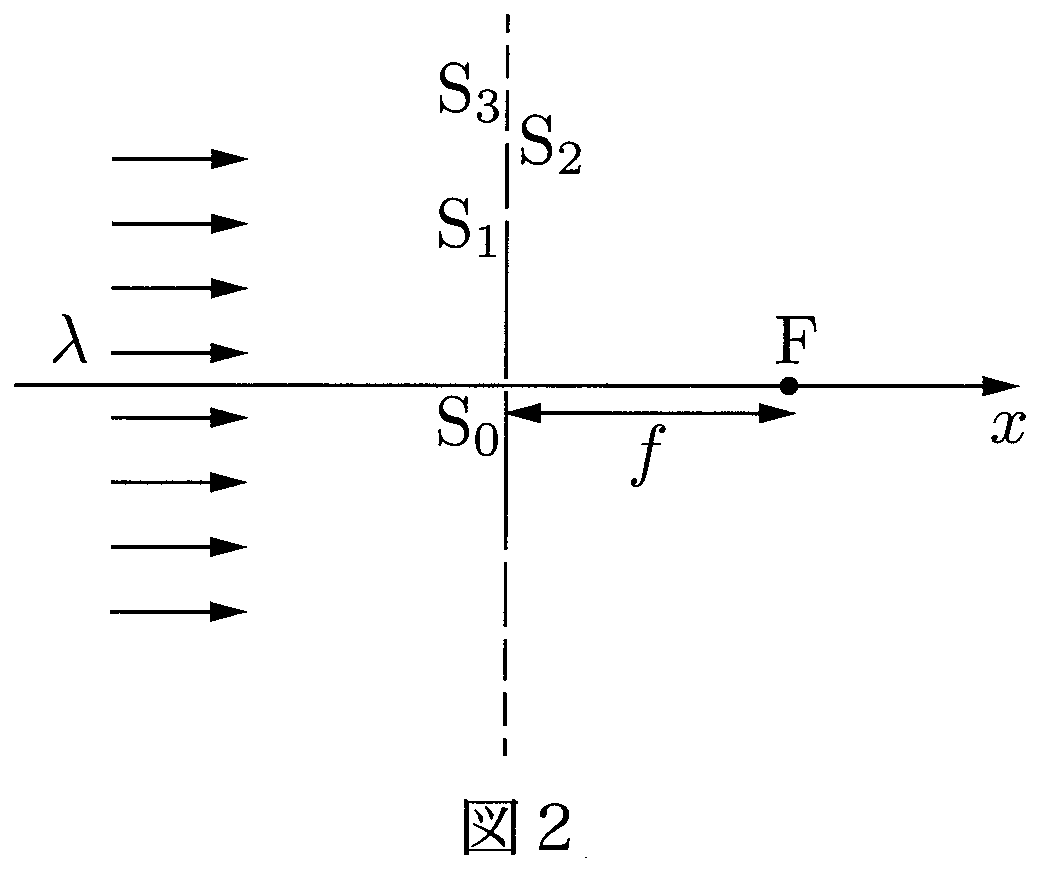
\includegraphics[keepaspectratio,width=58mm]{fig/n19_p60_zu2.png}
\end{zuright}
\begin{komon}
\ko{1} スリット$\mathrm{S}_m$の半径$r_m\U{m}$を求めよ．ただし，$\overline{\mathrm{OF}}=f\U{m}\gg r_N$とし，一次近似を利用して答えよ．
\end{komon}

\vspace{2mm}
\hspace{1zw}このスリットを利用して，以下のような実験を行った．
\begin{zuright}{58mm}
\begin{komon}
\ko{2} 空気中で，図3のように$x$軸上の$\overline{\mathrm{OA}}=a\U{m}$（ただし$a>f$）である点$\mathrm{A}$に波長$\lambda\U{m}$の点光源を置くと，$\mathrm{S_1}$, $\mathrm{S_2}$, $\cdots$, $\mathrm{S}_N$を通った光と$\mathrm{S_0}$を通った光が，それぞれ$\lambda$, $2\lambda$, $\cdots$, $N\lambda$の光路差を生じて強め合うような$x$軸上の点$\mathrm{B}$が存在する．$\overline{\mathrm{OB}}=b\U{m}$とするとき，$a$, $b$, $f$の間に成立する関係式を求めよ．ただし，$a$, $b\gg r_N$であるとする．
\end{komon}
\zusep
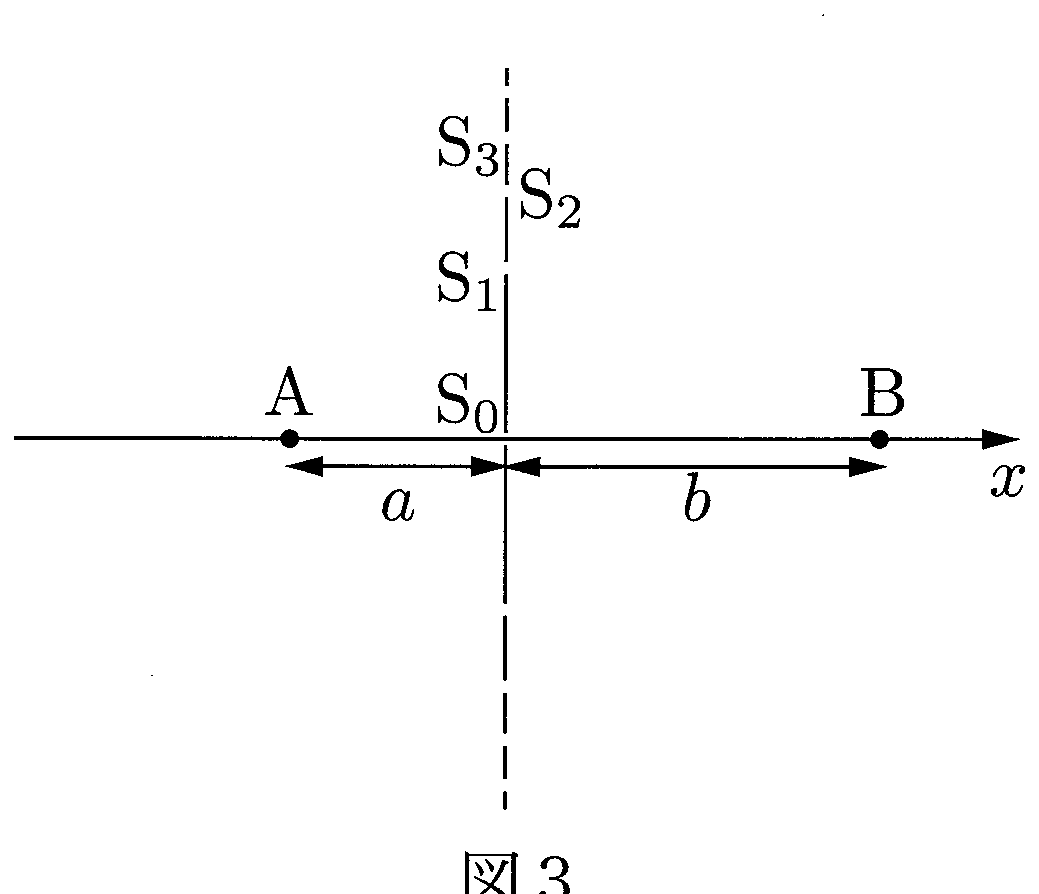
\includegraphics[keepaspectratio,width=58mm]{fig/n19_p60_zu3.png}
\end{zuright}

\begin{zuright}{58mm}
\begin{komon}
\ko{3} 図4のように，$x\geqq 0$の部分だけを水で満たし，$x$軸負の側から波長$\lambda\U{m}$の平行光線を当てると，空気中では$\mathrm{F}$であった光の強め合いの点が，$x$軸上の点$\mathrm{F^\prime}$へ移る．$\overline{\mathrm{OF^\prime}}=f^\prime\U{m}$とするとき，$f^\prime$を$f$および水の屈折率$n$を用いて表せ．ただし，$f^\prime\gg r_N$であるとする．
\end{komon}
\zusep
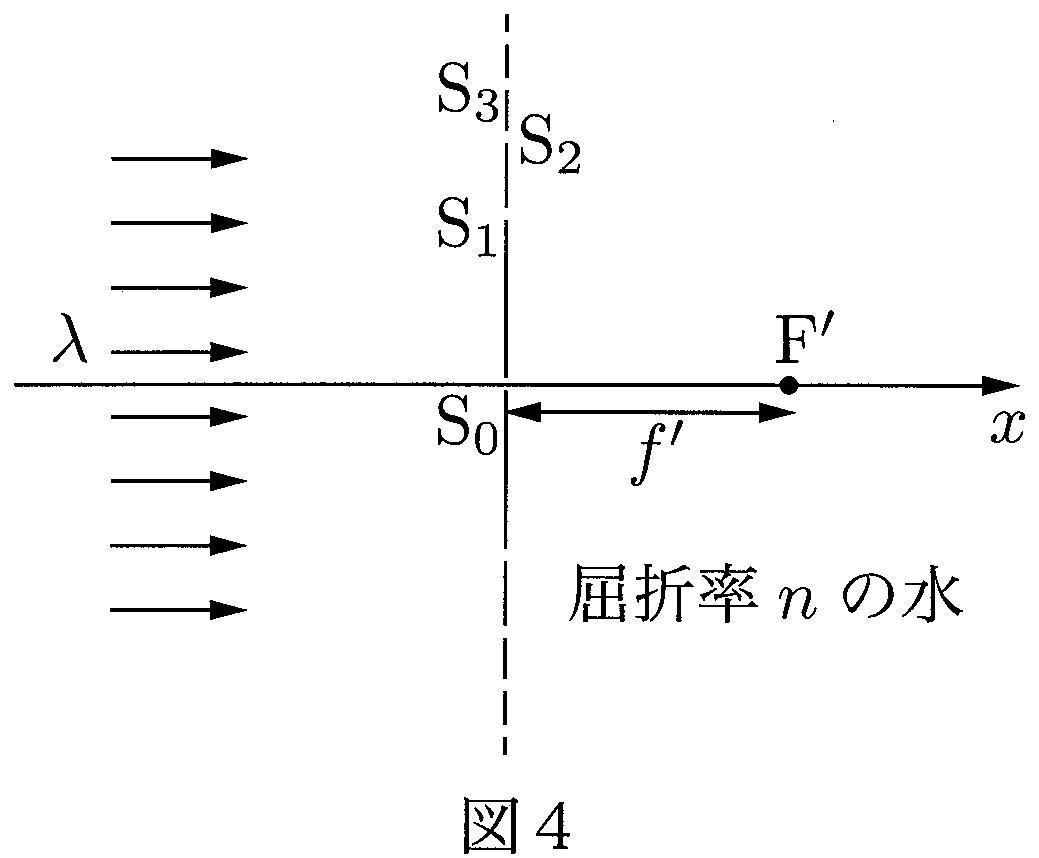
\includegraphics[keepaspectratio,width=58mm]{fig/n19_p60_zu4.png}
\end{zuright}

\Mon{マイケルソン干渉計}

% 図を58→78mmに拡大（58mmだと S/H/M1/M2/D/O/l1/l2 のラベルが読めない）。
% 同ページの下2/3が空いているので版面に余裕がある（2026-09-14）。
\begin{zuright}{78mm}
\hspace{1zw}波長$\lambda\U{m}$の単色光源$\mathrm{S}$，半透鏡（ハーフミラー）$\mathrm{H}$，反射鏡$\mathrm{M_1}$, $\mathrm{M_2}$，および光検出器$\mathrm{D}$を図のように配置する．光源$\mathrm{S}$から出た光は$45^\circ$に傾いて配置されたハーフミラー$\mathrm{H}$により二分され，ひとつはそのまま通過して反射鏡$\mathrm{M_1}$に向かい，もう一つは反射鏡$\mathrm{M_2}$に向かう．それぞれの鏡で反射された光は図の$x$, $y$軸上を逆向きに進んでハーフミラー$\mathrm{H}$に戻って光検出器$\mathrm{D}$に向かい，光検出器$\mathrm{D}$ではこの二つの光による干渉が見られる．

\hspace{1zw}ハーフミラー$\mathrm{H}$は反射光と透過光の強さが等しい半透明の平面鏡であり，その厚さは無視できるものとする．$\mathrm{M_1}$および$\mathrm{M_2}$は光軸に対して垂直に置かれているものとして以下の設問に答えよ．
\zusep
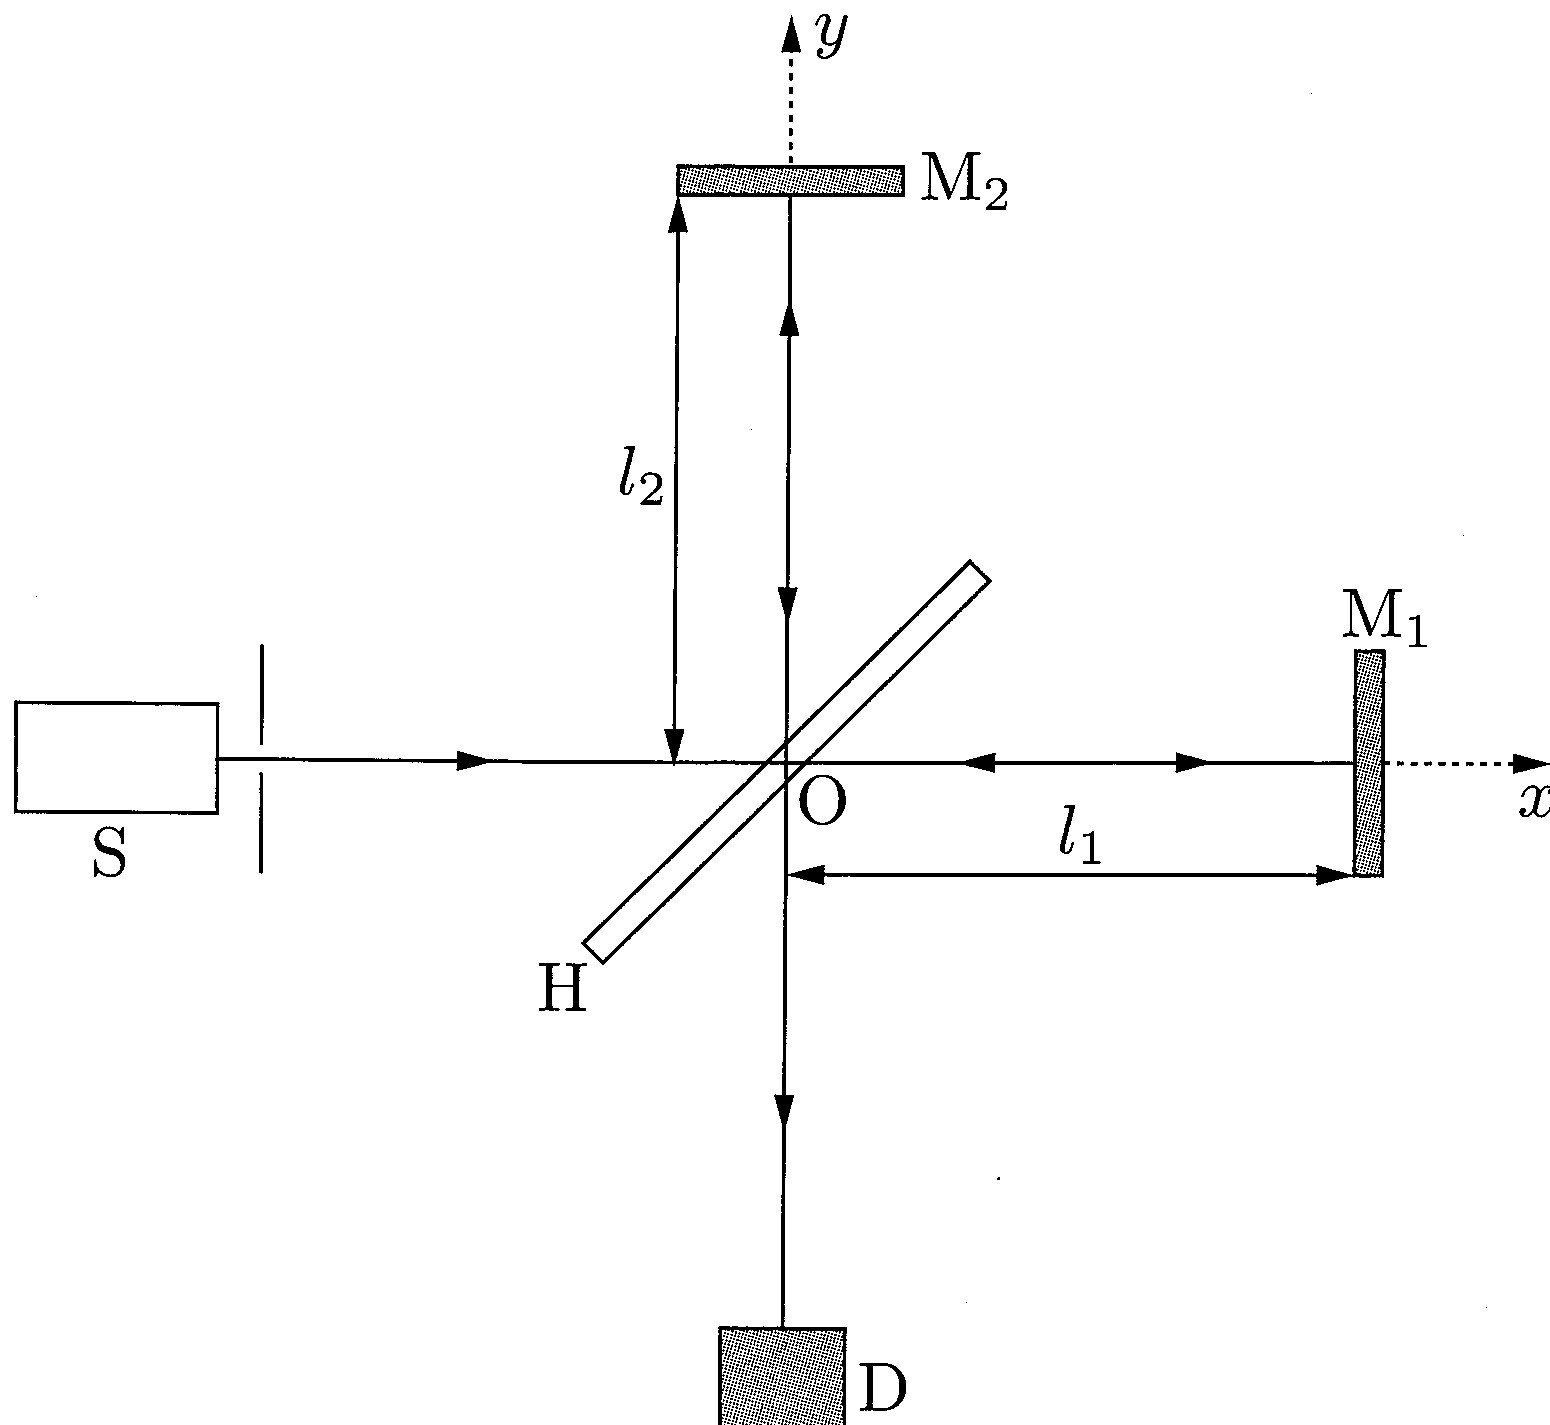
\includegraphics[keepaspectratio,width=78mm]{fig/n19_p61_michel.png}
\end{zuright}
\begin{komon}
\ko{1} $\overline{\mathrm{OM_1}}=l_1\U{m}$, $\overline{\mathrm{OM_2}}=l_2\U{m}$, $l_1>l_2$であるとき，光検出器$\mathrm{D}$に入射する光が強め合う条件を求めよ．
\ko{2} 反射鏡$\mathrm{M_1}$を$x$軸上で，(1)の条件を満たす強め合いの位置から距離$\Delta x\U{m}$だけゆっくりと遠ざけていったところ，その間に$\mathrm{D}$では光の弱め合い，強め合いが交互に起こり，動かし終わったところでちょうど$m$回目の明るい状態になった（初めの強め合いを0回目と数えるものとする）．移動距離$\Delta x$を，$m$, $\lambda$を用いて表せ．
\end{komon}

\Mon{反射光の干渉}

\begin{zuright}{62mm}
\hspace{1zw}コンパクトディスクに光が当たると虹のような色が見えるが，この原因について考えてみよう．コンパクトディスクは内部のアルミ箔に多数の溝が等間隔に刻まれているもので，光の反射板の役割を果たす．このうち，溝の部分に当たった光はさまざまな方向に乱反射して弱め合ってしまうが，溝によって隔てられた各平面部分からの反射によって強め合い・弱め合いが起こり，虹のような色が見える．
\zusep
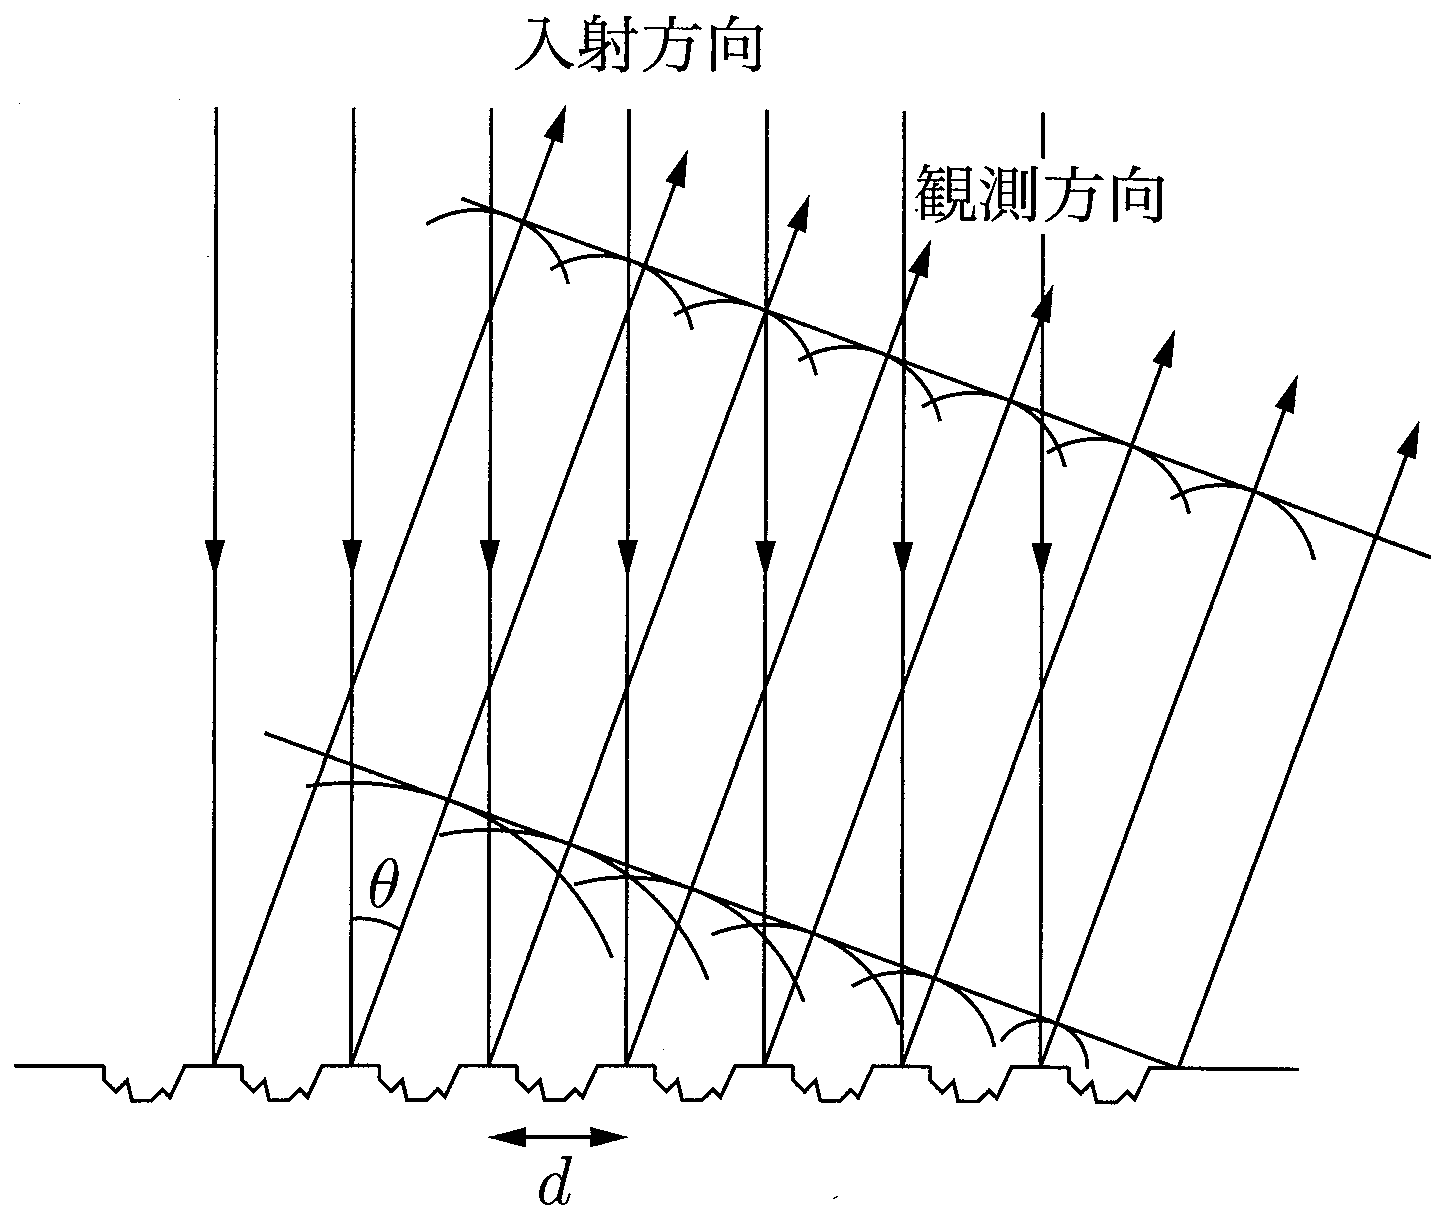
\includegraphics[keepaspectratio,width=62mm]{fig/n19_p62_cd.png}
\end{zuright}

\hspace{1zw}簡単のため，コンパクトディスクの面に対して垂直に光が入射した場合について考えると，溝によって隔てられた各平面部分からホイヘンスの原理に従って素元波が出て反射していき，それらが互いに干渉しあう．図1のように，反射板に対して垂直な入射方向に対して$\theta$の方向から光の強さを観測する．溝の平面部分の間隔を$d\U{m}$として，以下の設問に答えよ．
\begin{komon}
\ko{1} 入射光が波長$\lambda\U{m}$の単色光である場合の，光が強め合うための条件を$d$, $\theta$, $\lambda$および整数値$m$を用いて表せ．
\end{komon}

\vspace{2mm}
\hspace{1zw}入射光が$400\U{nm}$〜$700\U{nm}$（$1\U{nm}=10^{-9}\U{m}$）の範囲の可視光を含んだ白色光である場合を考える．コンパクトディスクのアルミ箔上には，溝が$1\U{cm}$あたり6250本だけ刻まれている．
\begin{komon}
\ko{2} 観測する方向$\theta$を，$0^\circ$から増加させていく．まず，$\theta=0^\circ$で強い反射がある．さらに$\theta$を大きくしていくと，角度$\theta_1$で強い光が見え始め，それは$\theta$の増加と共に色を変えながら角度$\theta_2$まで観測された．$\theta_1$, $\theta_2$のおおよその値を，下のグラフを参考にして求めよ．
       \begin{center}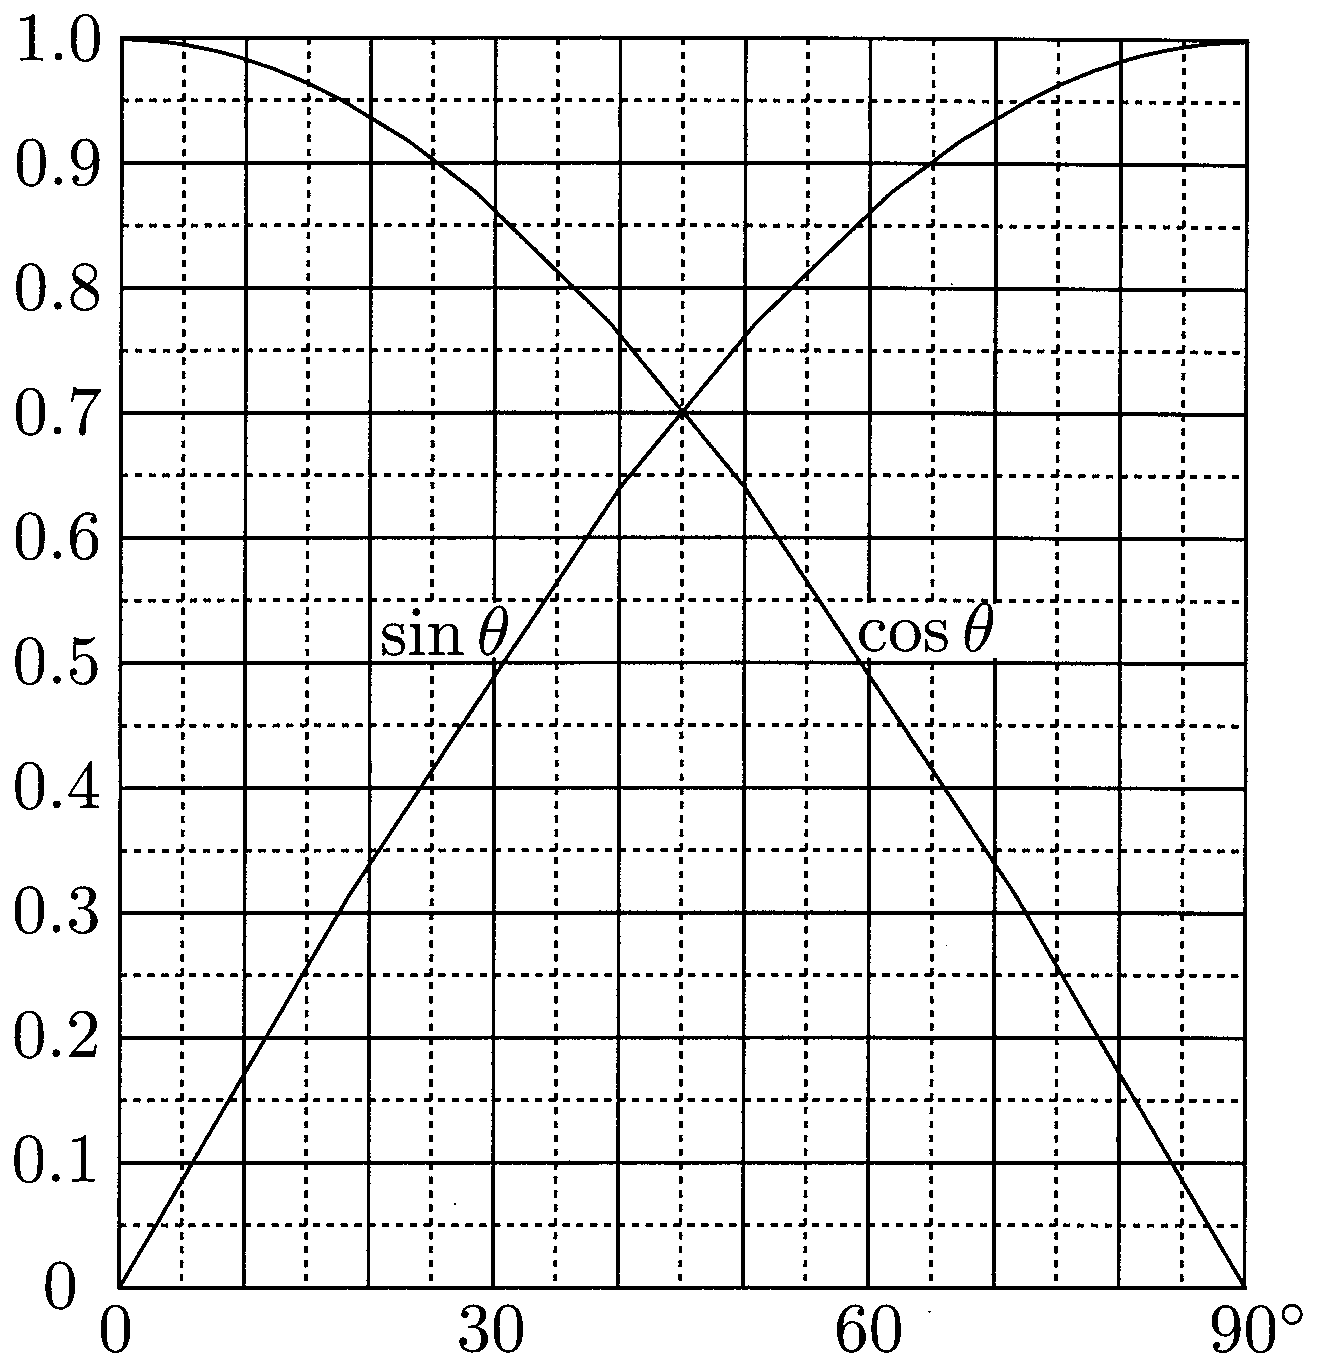
\includegraphics[keepaspectratio,width=76mm]{fig/n19_p62_graph.png}\end{center}
\ko{3} (2)で，観測方向$\theta$が$\theta_1$から$\theta_2$まで増加するとき，色が変化していく順番は以下のうちのいずれか．\\
       \hspace*{2zw}\MARU{1} 赤，黄，緑，青，紫\hspace{8mm}\MARU{2} 赤，緑，青，黄，紫\\
       \hspace*{2zw}\MARU{3} 紫，青，緑，黄，赤\hspace{8mm}\MARU{4} 紫，黄，青，緑，赤
\end{komon}


\newpage

\KaiTitle{第19回　薄膜・くさび・ニュートンリングの干渉}
\setlength{\columnseprule}{0.4pt}
\begin{multicols}{2}
\raggedcolumns

\Rank{A問題}
\MonN{54}{基本公式の確認}\par\nopagebreak
\begin{sisin}
光波干渉に関する基本問題である．(1)については簡単な図を描いて光路差を求めればよい．(2)については，座標軸を設定して明線位置を求める，という面倒な方法ではなく，{\gtfamily 隣り合う明線の光路差は$\lambda\U{m}$だけ異なる}という重要な事項を利用すれば簡単に求められることを覚えておくこと．
\end{sisin}
\KaiHead
\begin{komon}
\ko{1} 有機薄膜上面から入射して上面へ再び戻っていく光は，次図にあるように，有機膜上面で直接反射した光と，有機膜下面で反射した光の二つの干渉光である．
       \begin{center}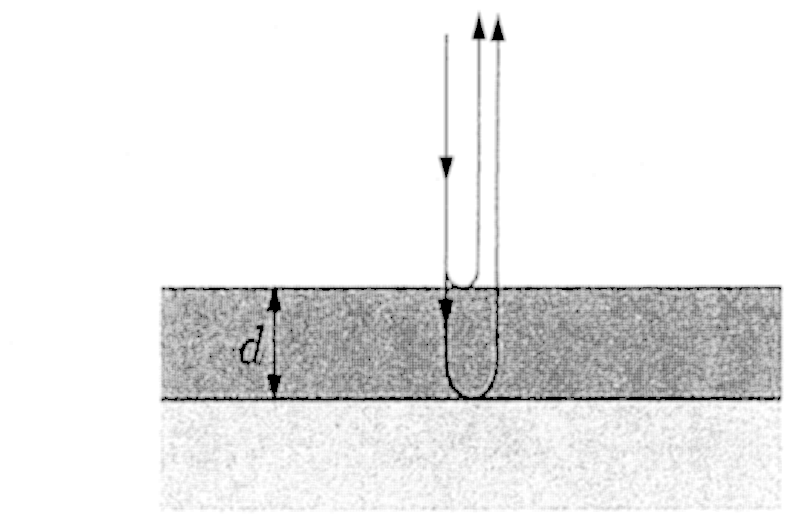
\includegraphics[keepaspectratio,width=56mm]{fig/n19_a54_film.png}\end{center}
       よって光路差は，往復分を考えて$n\times 2d\U{m}$である．また，屈折率を考えると，有機薄膜上面での反射のみ位相が$\pi$ずれる．よって，反射光が強め合うのは，整数値$m$を用いて
       \[2nd=m\lambda+\frac{\lambda}{2}\]
       の条件が満たされるときである．これを満たす最小の$d$は，$m=0$のときで，
       \[d=\frac{\lambda}{4n}\U{m}\Ans\]
\ko{2} 隣り合う二つの明線を考える．
       \begin{center}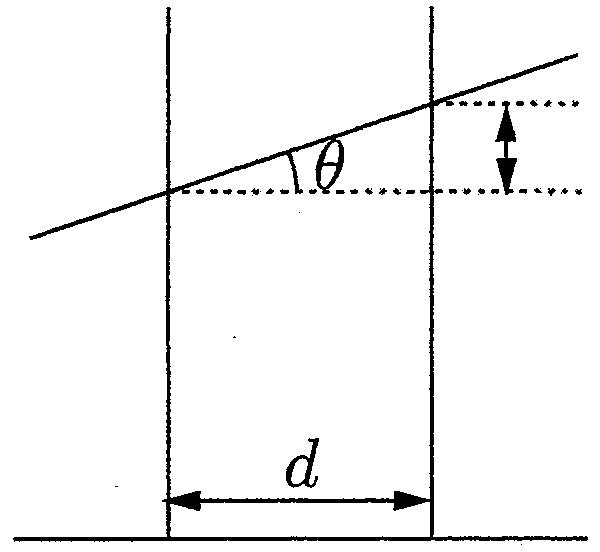
\includegraphics[keepaspectratio,width=34mm]{fig/n19_wedge_pitch.png}\end{center}
       隣り合う明線の間隔を$d\U{m}$とすると，この二つの位置の光路差の差は，図の縦の矢印の長さの2倍（往復分）であるから
       \[2\times d\tan\theta\U{m}\]
       であるが，隣り合う二つの明線位置の光路差は$\lambda\U{m}$だけ違うので，
       \[2\times d\tan\theta=\lambda\]
       が成立する．これを解いて，明線間隔は
       \[d=\frac{\lambda}{2\tan\theta}\U{m}\]
       であり，$\tan\theta\fallingdotseq\theta$と近似すると，
       \[d\fallingdotseq\frac{\lambda}{2\theta}\U{m}\Ans\]
\end{komon}

\Rank{B問題}
\MonN{55}{光学的距離（ジャマンの実験）}\par\nopagebreak
\begin{sisin}
光学的距離を用いて光の干渉を考える問題である．屈折率によって波の波長は変化するため，経路によって何波長分ずれるのかは幾何学的な距離からは考えにくい．{\gtfamily 屈折率$\times$経路長}という光学的距離を考えれば真空中での波長の値そのままを利用して何波長分ずれるのかを考えることが出来るため便利である．

本問の場合，上の経路と下の経路で食い違っているのは管$\mathrm{T_1}$, $\mathrm{T_2}$の部分で，ここで何波長分かのずれが生じる．よってこの部分の光路差から光の強め合い・弱め合いを議論しよう．ただし，管$\mathrm{T_1}$の光路長を求めてそれをそのまま光路差にしないように注意．管$\mathrm{T_2}$の方の光路長も考えなければならない．
\end{sisin}
\KaiHead
\begin{komon}
\ko{1} 管$\mathrm{T_1}$, $\mathrm{T_2}$のそれぞれを通る経路は，管$\mathrm{T_1}$, $\mathrm{T_2}$の内部を通る部分を除いては距離・媒質共に全く同一であるので，波のずれを生じるのは管$\mathrm{T_1}$, $\mathrm{T_2}$の内部の部分である．よって二つの光の光路差は，管$\mathrm{T_1}$, $\mathrm{T_2}$の部分のみについて考えればよい．

       このとき，管$\mathrm{T_1}$, $\mathrm{T_2}$の内部の光路長はそれぞれ
       \[\mathrm{T_1}:1\times l\U{m},\hspace{3mm}\mathrm{T_2}:n\times l\U{m}\]
       であるから，二つの光の光路差は，
       \[(n-1)l\U{m}\Ans\]
\ko{2} $\mathrm{Q}$点で光が強め合うのは，二つの光の光路差が真空中の波長$\lambda\U{m}$の整数倍になっているときである．よって，
       \[(n-1)l=m\lambda,\ m\geqq 0\]
       が成立するときであり，これを解いて，
       \[n=1+m\frac{\lambda}{l},\ m\geqq 0\Ans\]
\ko{3} はじめは管$\mathrm{T_2}$内は真空であったから$n=1$であり，このとき強め合いの条件を満たしていた．これは(2)の答えの式の$m=0$の場合に対応している．

       このあと気体を注入して圧力を増加させていくと気体の屈折率は徐々に増加していく．増加するにつれて弱め合い，強め合いを繰り返して$1.00\times 10^5\U{Pa}$になったときに50回目の強め合いとなったのだから，このときは$m=50$の強め合いに対応していると考えられる．

       以上より，この気体の圧力が$1.00\times 10^5\U{Pa}$のときの気体の絶対屈折率は，
       \begin{align*}
       n&=1+50\times\frac{\lambda}{l}=1+50\times\frac{5.90\times 10^{-7}}{1.00\times 10^{-1}}\\
        &=1.000295\Ans
       \end{align*}
       \begin{bsHosoku}{参考}
       気体の圧力の増加に伴って屈折率が増大していくのは，媒質（気体）の密度が高くなっていくためである．同じ物質であれば密度が高いほど屈折率は高い．
       \end{bsHosoku}
\ko{4} 気体の圧力に比例して強め合い・弱め合いが交互に起こること，および強め合いが起こる気体の屈折率が$n=1+m\times$(定数)の式で表されることから，気体の絶対屈折率は圧力に対して一次関数的に変化していることが分かる．気体の圧力が$0.00\U{Pa}$（真空）のときは$n=1$，気体の圧力が$1.00\times 10^5\U{Pa}$のときは$n=1.000295$であったことに注意して式を作ると，
       \[n=1+0.000295p\Ans\]
       \begin{bsHosoku}{参考}
       このように一般に気体の屈折率はほぼ1であるため，光線の屈折から気体の屈折率を測定するのはほぼ不可能である．本問のように，光波の干渉をうまく利用すると気体の屈折率を精密に求めることができる．
       \end{bsHosoku}
\end{komon}

\MonN{56}{くさびガラスの干渉}\par\nopagebreak
\begin{sisin}
隣り合う二つの明線（もしくは暗線）の間隔を，A問題で学んだ考え方で先に求めてしまうのも一つの手であるが，本問の(1)〜(3)の場合は明線間隔だけではなく，$\mathrm{A}$側から数えて$m$番目の明線の位置について問われているので，\MARU{1}光路差を求める，\MARU{2}反射による位相のずれを調べる，\MARU{3}明線条件を定める，というオーソドックスな手法で順番に考えて明線位置を決めよう．

ただし(4)については，液体の屈折率とガラス$\mathrm{G_1}$および$\mathrm{G_2}$の屈折率の大小関係次第で\MARU{2}の反射による位相のずれの条件がさまざまに変化しうるので，A問題で学んだ考え方を用いて明線間隔を求めてしまった方がラクである．
\end{sisin}
\KaiHead
\begin{komon}
\ko{1} $\mathrm{A}$から距離$y\U{m}$の位置での空気層の厚さを$a\U{m}$とすると，この位置では上方から見るとガラス$\mathrm{G_2}$の下面で反射した光とガラス$\mathrm{G_1}$の上面で反射した光とが光路差$2a\U{m}$で干渉する．
       \begin{center}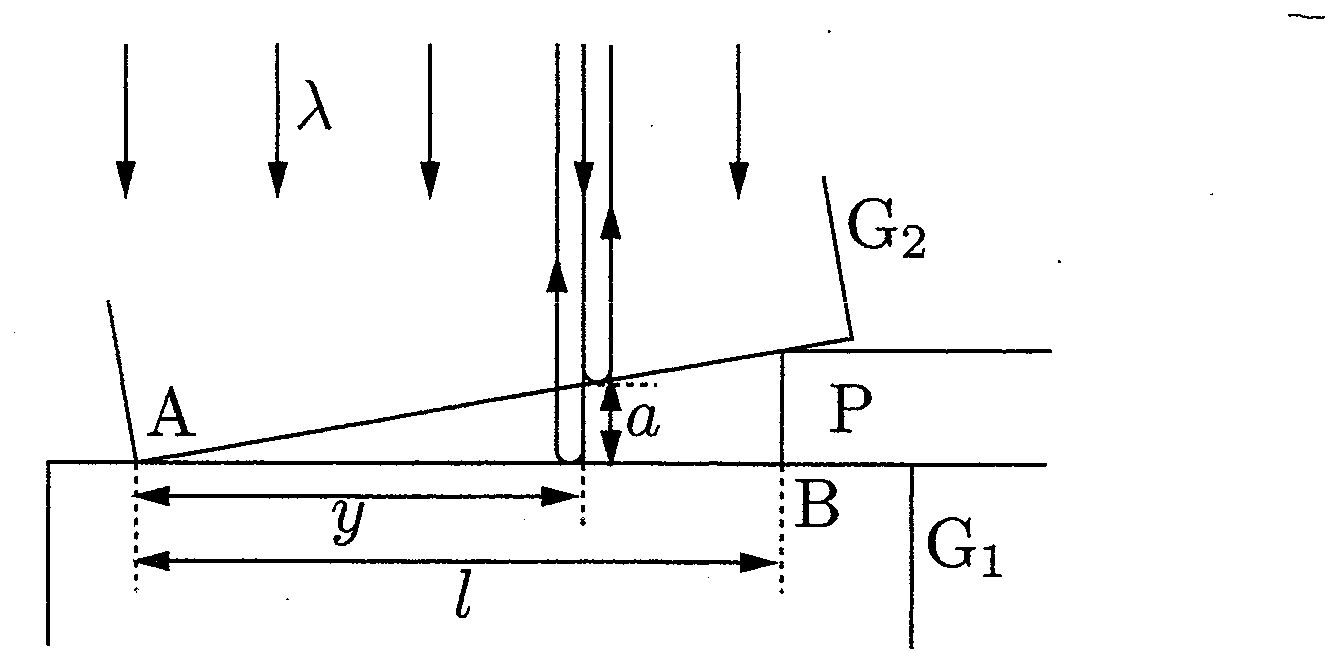
\includegraphics[keepaspectratio,width=58mm]{fig/n19_a56_wedge.png}\end{center}
       ガラスの屈折率$>$空気の屈折率であるから，ガラス$\mathrm{G_2}$の下面での反射では位相はずれず，ガラス$\mathrm{G_1}$の上面での反射では位相が$\pi$ずれる．よって，光路差が1波長の整数倍＋半波長のとき，この二つの光は強め合う．よって，明線が出来るのは光路差が
       \[2a=i\lambda+\frac{\lambda}{2}\hspace{3mm}(i\text{は整数値})\]
       の条件を満たすとき，すなわち空気層の厚さが
       \[a=i\frac{\lambda}{2}+\frac{\lambda}{4}\hspace{3mm}(i\text{は整数値})\]
       となる位置である．$\mathrm{A}$に近い位置の方が$a$が小さいので，最も$\mathrm{A}$に近い明線は空気層の厚さが$a=\dfrac{\lambda}{4}$（$i=0$に対応）となる位置で，これが1番目の明線である．2番目の明線は空気層の厚さが$a=\dfrac{\lambda}{2}+\dfrac{\lambda}{4}$（$i=1$に対応）となる位置である．同様に，$m$番目の明線の位置は空気層の厚さが
       \[a=(m-1)\frac{\lambda}{2}+\frac{\lambda}{4}\hspace{3mm}(i=m-1\text{に対応})\]
       となる位置である．$a$を$d$に取り替えて式を整理して，
       \[d=\frac{(2m-1)\lambda}{4}\U{m}\Ans\]
\ko{2} 紙の厚さを$D\U{m}$とすると，$a$, $y$の関係は幾何学的関係より
       \[y:a=l:D\]
       であるから，$y=\dfrac{l}{D}a\U{m}$である．強め合うのは$a=i\dfrac{\lambda}{2}+\dfrac{\lambda}{4}$のときであるから，明線が出来るのは$\mathrm{A}$から
       \[y=\frac{l}{D}\left(i\frac{\lambda}{2}+\frac{\lambda}{4}\right)\U{m}\hspace{3mm}(i\text{は整数値})\]
       の距離の位置である．よって明線間隔は，$i$をひとつずらして差し引くことにより，
       \begin{align*}
       b&=\frac{l}{D}\left\{(i+1)\frac{\lambda}{2}+\frac{\lambda}{4}\right\}-\frac{l}{D}\left(i\frac{\lambda}{2}+\frac{\lambda}{4}\right)\\
        &=\frac{l\lambda}{2D}
       \end{align*}
       である．これを解いて，
       \[D=\frac{l\lambda}{2b}\U{m}\Ans\]
\ko{3} (1)より，暗線が出来るのは光路差が1波長の整数倍となるところであり，
       \[2a=i\lambda\hspace{3mm}(i\text{は整数値})\]
       の条件が満たされる位置である．$y=\dfrac{l}{D}a\U{m}$の関係式より，$\mathrm{A}$からの距離が
       \[y=i\frac{l\lambda}{2D}\U{m}\]
       となる位置が暗線となる．$\mathrm{A}$の位置は$i=0$の暗線に対応しているので，$\mathrm{B}$の位置が41本目の暗線になるには$\mathrm{B}$の位置（$y=l\U{m}$）が$i=40$の暗線になればよい．よって，
       \[l=40\times\frac{l\lambda}{2D}\U{m}\]
       これを解いて紙の厚さを求めると，
       \[D=40\times\frac{\lambda}{2}=1.2\times 10^{-5}\U{m}\Ans\]
\ko{4} この液体の屈折率を$n$とおき，ガラス$\mathrm{G_2}$の傾き角を$\theta$とおく．次図のような隣り合う二つの明線位置を考える．
       \begin{center}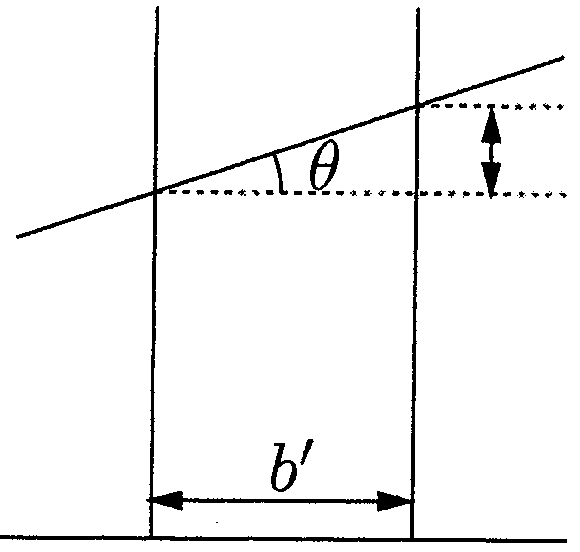
\includegraphics[keepaspectratio,width=34mm]{fig/n19_wedge_pitch_liquid.png}\end{center}
       この二つの位置の経路差の差は，図の縦の矢印の長さの2倍（往復分）であるから，この二つの位置の光路差の差は
       \[n\times 2b^\prime\tan\theta\U{m}\]
       だけ異なる．隣り合う二つの明線位置の光路差は$\lambda\U{m}$だけ違うので，
       \[n\times 2b^\prime\tan\theta=\lambda\]
       が成立する．また，ガラス$\mathrm{G_2}$の傾き角は$\tan\theta=\dfrac{D}{l}$であるから，
       \[b^\prime=\frac{l\lambda}{2nD}\U{m}\]
       である．また(2)より$D=\dfrac{l\lambda}{2b}$であるから，この2式より$D$を消去すると，
       \[n=\frac{b}{b^\prime}\Ans\]
\end{komon}

\MonN[\Sitei]{57}{ニュートンリング}\par\nopagebreak
\begin{sisin}
ニュートンリングに関する総合問題であるが，まず{\gtfamily 空気層の厚さの求め方}をよく覚えておくこと．テキストでは円周角と相似を利用して求める方法を示してあるが，ここでは三平方の定理をもとに近似する方法を示す．

(3)では，関数$y=\sqrt{x}$が上に凸の単調増加関数であることを利用すれば簡単に理解できる．

平凸レンズの移動によって明環・暗環がどのように動くのかは，{\gtfamily 同じ経路差（すなわち空気厚）を持つ点がどちらの方向に移動するのかを考えよ．}

また反射光を下面から観察する場合には，リングを直接通り抜けていく光と，空気層の部分を往復してから下へ抜ける光とが干渉する．反射による位相のずれの条件を間違えないように注意．
\end{sisin}
\KaiHead
\begin{komon}
\ko{1} 次の図の三角形$\mathrm{ABC}$に対して三平方の定理を適用する．
       \begin{center}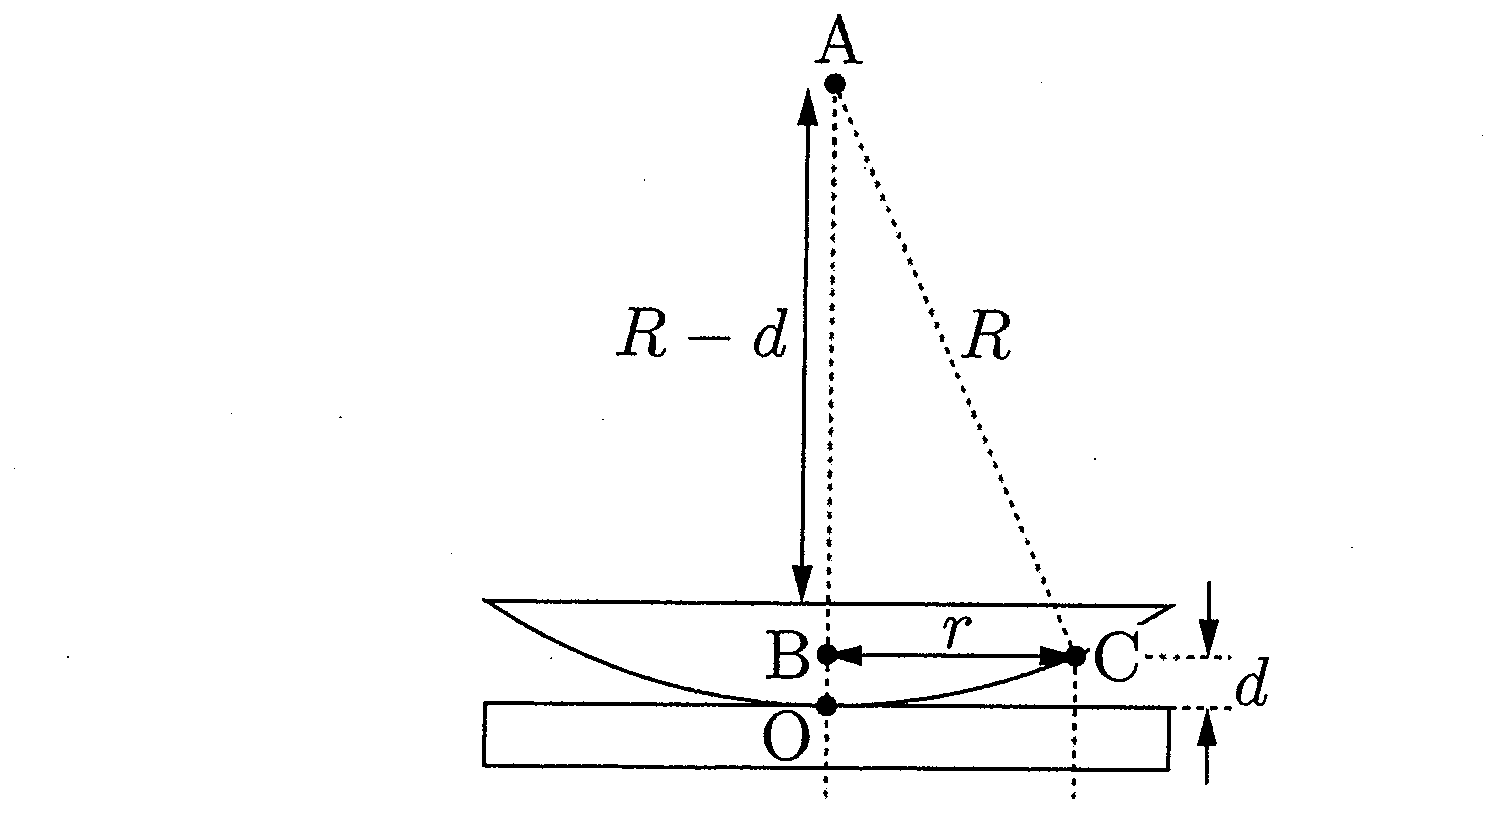
\includegraphics[keepaspectratio,width=54mm]{fig/n19_a57_abc.png}\end{center}
       この図において，$\overline{\mathrm{AB}}=R-d\U{m}$であるから，
       \[R^2=(R-d)^2+r^2\]
       が成立し，これを$d$について解くと
       \[d=R-\sqrt{R^2-r^2}\]
       となる．ルート部分を$R\gg r$であることに基づいて一次近似すると，
       \begin{align*}
       \sqrt{R^2-r^2}&=R\left\{1-\left(\frac{r}{R}\right)^2\right\}^{\frac{1}{2}}\\
       &\fallingdotseq R\left\{1-\frac{1}{2}\left(\frac{r}{R}\right)^2\right\}
       \end{align*}
       であるから，
       \[d\fallingdotseq R-\left(R-\frac{r^2}{2R}\right)=\frac{r^2}{2R}\U{m}\Ans\]
\ko{2} 上から見た場合には，平凸レンズ下面で反射した光と，平板ガラスの上面で反射した光とが干渉して見える．
       \begin{center}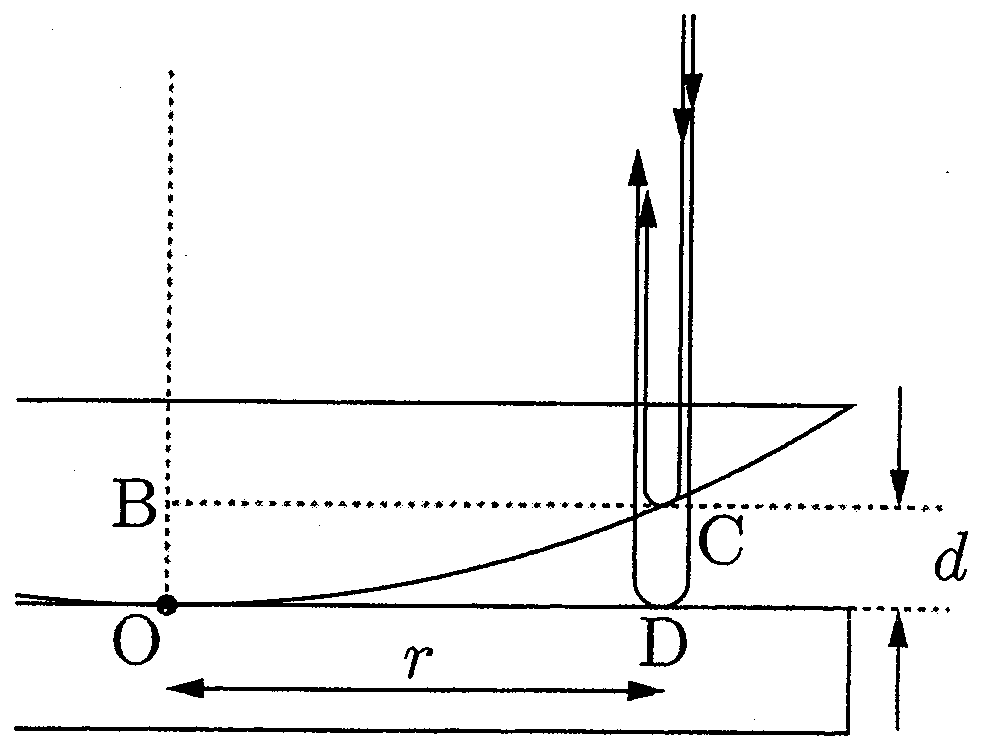
\includegraphics[keepaspectratio,width=48mm]{fig/n19_a57_top.png}\end{center}
       よって，この二つの光は光路差$2d\U{m}$で干渉する．反射による位相のずれは，空気の屈折率$<$ガラスの屈折率であるから，$\mathrm{C}$点での反射では位相がずれず，$\mathrm{D}$点での反射では位相が$\pi$ずれる．よって，合わせて反射によって位相は$\pi$ずれるので，
       \[2d=\frac{r_m^{\,2}}{R}=m\lambda\ \text{のとき弱め合い}\]
       \[2d=\frac{r^{\prime\,2}_m}{R}=m\lambda-\frac{1}{2}\lambda\ \text{のとき強め合い}\]
       となる．よってこれらを解いて，
       \[\left\{\begin{array}{l}\text{暗環の半径：}r_m=\sqrt{mR\lambda}\U{m}\\[2mm]\text{明環の半径：}r^\prime_m=\sqrt{\left(m-\dfrac{1}{2}\right)R\lambda}\U{m}\end{array}\right.\]
       \[\Ans\]
       \begin{chuu}
       強め合いの条件式で$\dfrac{r^{\prime\,2}_m}{R}=m\lambda+\dfrac{1}{2}\lambda$と置かなかったのは，これだと一番内側の明環が$m=1$に対応しなくなってしまうからである．強め合いの条件は，整数値$i$を用いて
       \[\frac{r^2}{R}=i\lambda+\frac{1}{2}\lambda\]
       と書け，これを解いて
       \[r=\sqrt{\left(i+\frac{1}{2}\right)R\lambda}\U{m}\hspace{2mm}(i\text{は整数値})\]
       となる．よって，明環の半径を書き下すと
       \[r=\sqrt{\frac{1}{2}R\lambda},\ \sqrt{\frac{3}{2}R\lambda},\ \sqrt{\frac{5}{2}R\lambda},\ \cdots\]
       となるので，一番内側の明環を$m=1$に対応させるには，強め合いの条件式を$2d=\dfrac{r^{\prime\,2}_m}{R}=m\lambda-\dfrac{1}{2}\lambda$と置けばよい．分かりにくい場合には，まずいったん整数値$i$を用いて$\dfrac{r^2}{R}=i\lambda+\dfrac{1}{2}\lambda$としておき，これを$m$で表すように書き換えればよい．
       \end{chuu}
\ko{3} 例えば暗環について考えると，暗環の半径は
       \[r_m=\sqrt{R\lambda}\sqrt{m}=(\text{定数値})\times\sqrt{m}\]
       という形になっている．ここで，関数$y=\sqrt{x}$を考えると，これは上に凸の単調増加関数であるから，$\sqrt{m}$を$y=\sqrt{x}$のグラフ上で表すと次図のようになり，これは$m$が増加するにつれて明らかに間隔が狭まっていく．
       \begin{center}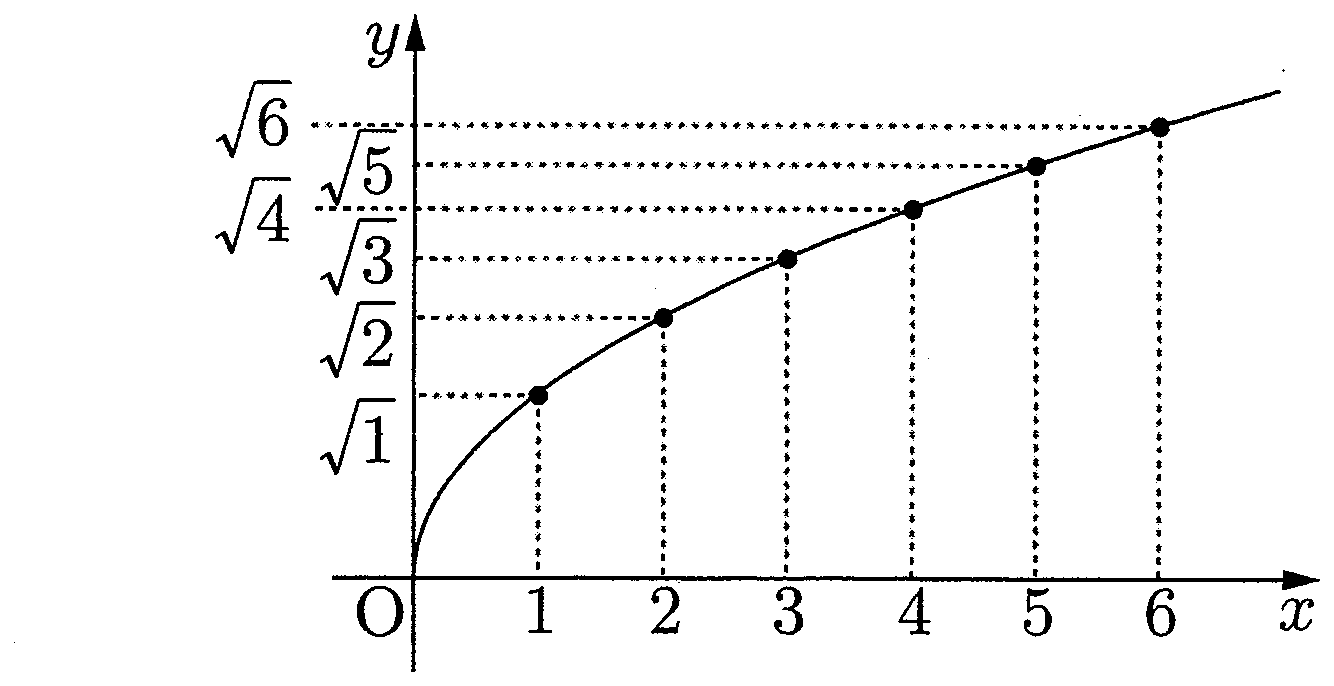
\includegraphics[keepaspectratio,width=54mm]{fig/n19_a57_sqrt.png}\end{center}
       明環についても全く同様に考えられるので，環の間隔は外側にいくほど狭まっていく．\hspace*{\fill}\Ans
       \begin{bsHosoku}{参考}
       純粋に数学的に示そうとすると以下のようになる．$r_{m+1}-r_m$を計算すると，
       \begin{align*}
       r_{m+1}-r_m&=\sqrt{R\lambda}\left(\sqrt{m+1}-\sqrt{m}\right)\\
       &=\frac{\sqrt{R\lambda}}{\sqrt{m+1}+\sqrt{m}}
       \end{align*}
       となるが，これと$r_m-r_{m-1}$を比較すると，
       \begin{align*}
       &\frac{1}{r_{m+1}-r_m}-\frac{1}{r_m-r_{m-1}}\\
       &=\frac{1}{\sqrt{R\lambda}}\Big\{\left(\sqrt{m+1}+\sqrt{m}\right)\\
       &\hspace{14mm}-\left(\sqrt{m}+\sqrt{m-1}\right)\Big\}\\
       &=\frac{1}{\sqrt{R\lambda}}\left(\sqrt{m+1}-\sqrt{m-1}\right)>0
       \end{align*}
       であるから，
       \[\frac{1}{r_{m+1}-r_m}>\frac{1}{r_m-r_{m-1}}\hspace{2mm}(>0)\]
       である．よって，
       \[r_{m+1}-r_m<r_m-r_{m-1}\]
       となり，暗環の間隔は外側へいくほど（すなわち$m$が大きくなるほど）狭くなることが分かる．
       \end{bsHosoku}
\ko{4} 中心から数えて8番目の明環とは，(2)の干渉条件式である
       \[2d=m\lambda-\frac{1}{2}\lambda\]
       の$m=8$に対応するものである．よって，この位置でのすき間の間隔は，
       \[d=\frac{1}{2}\left(8\times\lambda-\frac{1}{2}\lambda\right)\fallingdotseq 2.1\times 10^{-6}\U{m}\Ans\]
       また，この明環の半径は(2)の答えの$r^\prime_m$の$m=8$の場合であるから，
       \[5.0\times 10^{-3}=\sqrt{\left(8-\frac{1}{2}\right)R\times 5.5\times 10^{-7}}\]
       が成立し，これを解いて，レンズの曲率半径は，
       \[R\fallingdotseq 6.1\U{m}\Ans\]
\ko{5} 平凸レンズを持ち上げていくと，同じ空気厚を持つ点は，次図に示したように中心$\mathrm{O}$に向かってずれていく．
       \begin{center}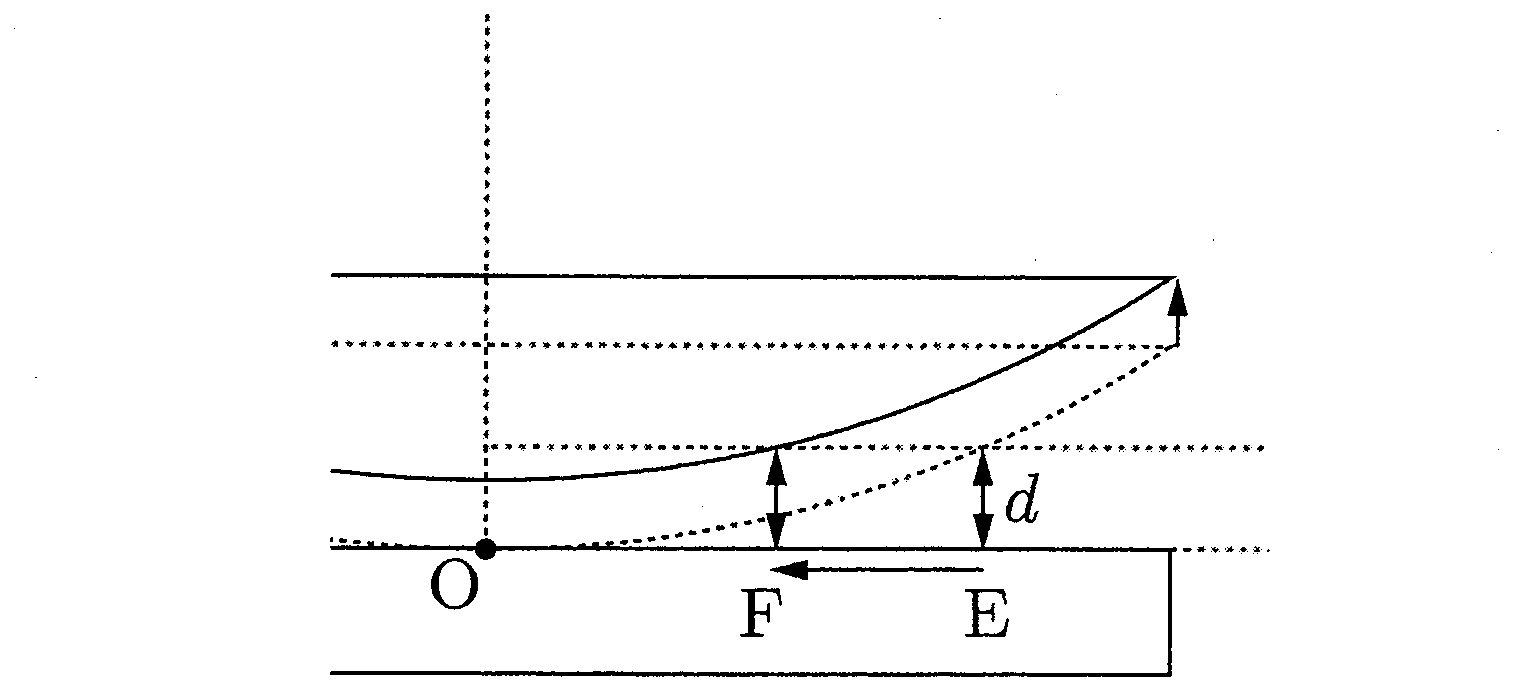
\includegraphics[keepaspectratio,width=58mm]{fig/n19_a57_lift.png}\end{center}
       例えばもともと$\mathrm{E}$点が暗線だったとする．平凸レンズを上に持ち上げると，上図にあるように同じ空気厚の点は左の$\mathrm{F}$点へずれるので，この暗線は$\mathrm{F}$の位置へとずれることになる．すなわち，明環・暗環は{\gtfamily 中心へ向かって移動する．}\hspace*{\fill}\Ans

       また，平凸レンズをさらに上に持ち上げていくと同じ空気厚を持つ点は中心まで移動したのち，なくなる．すなわち，明環・暗環は{\gtfamily 中心まで移動したのち消失する．}\hspace*{\fill}\Ans
\ko{6} 中心位置に着目すると，もともと中心は暗点であった．5本分だけリングが中心に向かって移動したのだから，平凸レンズを上に持ち上げたことにより，中心位置は元の$m=5$の暗環の位置の空気厚になったことが分かる（次図参照）．
       \begin{center}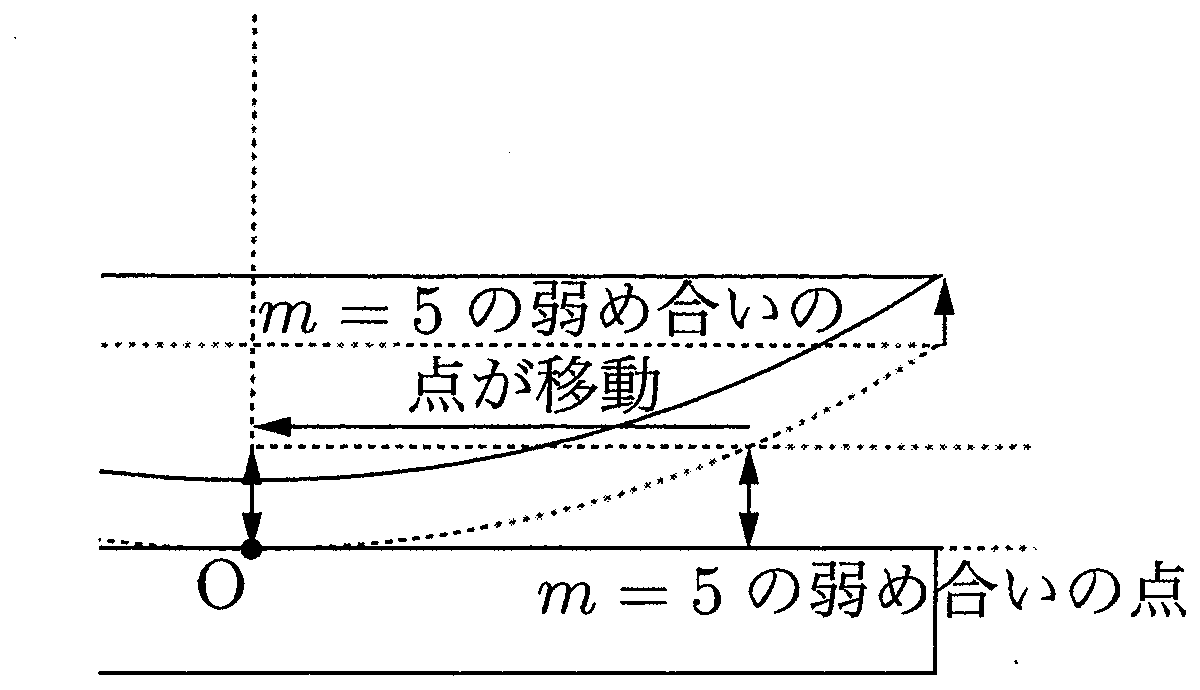
\includegraphics[keepaspectratio,width=58mm]{fig/n19_a57_lift2.png}\end{center}
       よって，平凸レンズを持ち上げた距離は，最初のときの$m=5$の暗環（弱め合い）の位置の空気厚分である．(2)より，この位置では
       \[2d=5\lambda\]
       であるから，
       \[d=\frac{5}{2}\lambda\U{m}\Ans\]
       だけ平凸レンズを持ち上げた．
\ko{7} 光を下面から観察する場合には，次図のように，リングを直接通り抜けていく光と，空気層の部分を往復してから下へ抜ける光とが干渉して強め合い・弱め合いを起こす．
       \begin{center}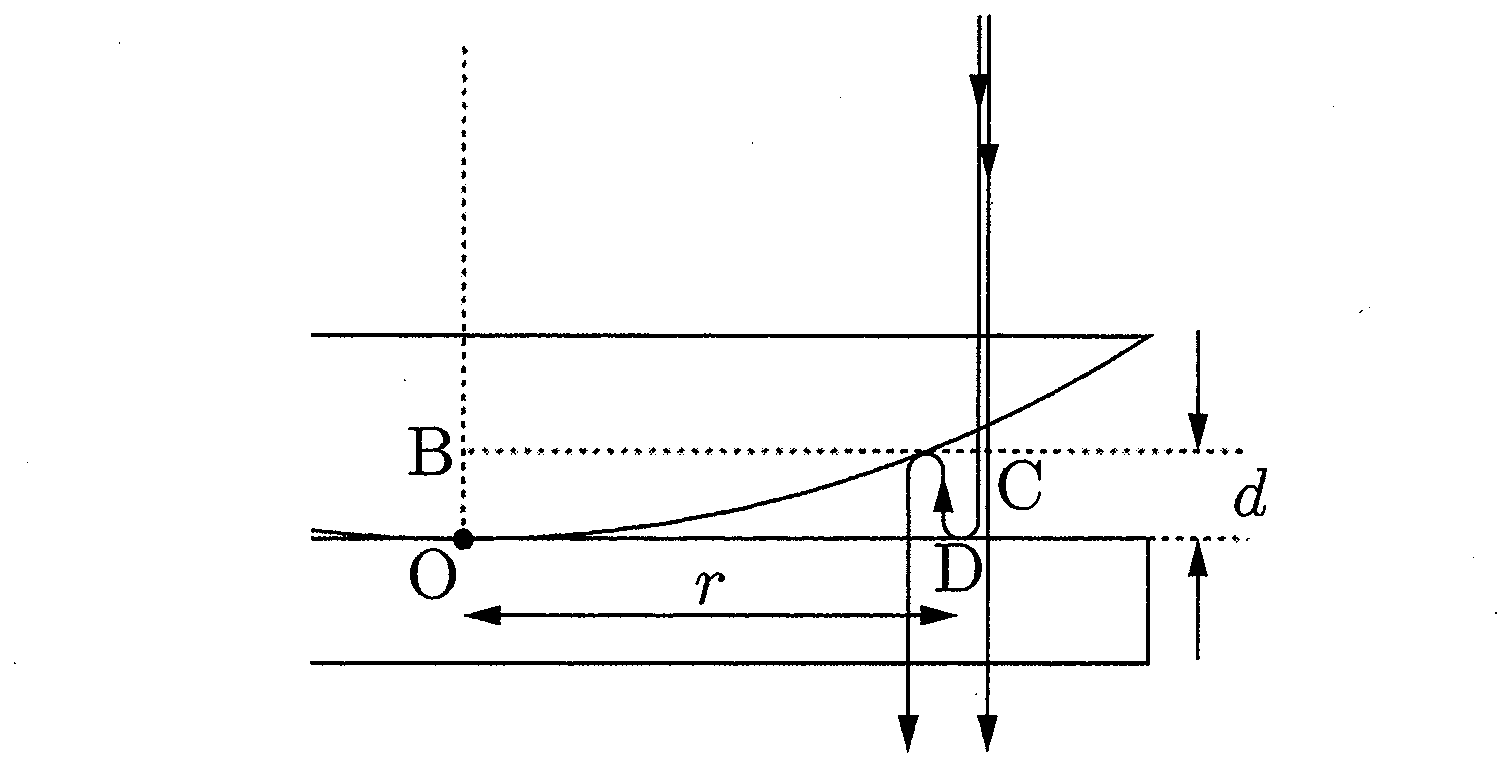
\includegraphics[keepaspectratio,width=58mm]{fig/n19_a57_under.png}\end{center}
       よって，前図のように下方向へ抜ける光は経路差$2d\U{m}$で干渉する．反射による位相のずれは，空気の屈折率$<$ガラスの屈折率であるから，$\mathrm{D}$点での反射では位相が$\pi$ずれ，その後の$\mathrm{C}$点での反射でも位相が$\pi$ずれる．よって，合わせて反射によって位相は$2\pi$ずれるので，
       \[2d=\frac{r^{\prime\,2}_m}{R}=m\lambda\ \text{のとき強め合い}\]
       \[2d=\frac{r_m^{\,2}}{R}=m\lambda-\frac{1}{2}\lambda\ \text{のとき弱め合い}\]
       となる．よってこれらを解いて，
       \[\left\{\begin{array}{l}\text{明環の半径：}r^\prime_m=\sqrt{mR\lambda}\U{m}\\[2mm]\text{暗環の半径：}r_m=\sqrt{\left(m-\dfrac{1}{2}\right)R\lambda}\U{m}\end{array}\right.\]
       \[\Ans\]
       \begin{chuu}
       上では$\mathrm{CD}$間を一往復してから下へ抜ける光について考えたが，2往復，3往復するような光は通常は考える必要がない．反射の際に光は透過光と反射光とに分かれるため，2往復，3往復するような光は1往復の光に比べて強度が小さい．よって，最初の1往復分の光についてのみ考えれば十分である．

       また，上から見た場合と下から見た場合とでは明環・暗環の位置がちょうど逆になっている．(7)の解答のように丁寧に考えればこれは明らかであるが，直観的には，上から照射した光は上へ反射する分と下へ抜ける分とに分かれるので，例えば上へ強め合って反射する場合には下には透過せずに暗環になる，と考えると分かりやすい．
       \end{chuu}
\end{komon}

\MonN[\Sitei]{58}{平行薄膜による干渉}\par\nopagebreak
\begin{sisin}
$\mathrm{C}$点を油と水の境界面に対して折り返してホイヘンスの原理を利用し，光路差$2nd\cos r\U{m}$を導く，というのは基本中の基本．説明方法まで含めて必ず覚えておくこと，また屈折率$n$をかけ忘れないように注意せよ．
\end{sisin}
\KaiHead
\begin{komon}
\ko{1} この光線は平行光線であるから，次図の$\mathrm{A}$, $\mathrm{A^\prime}$の点では位相が揃っている．ホイヘンスの原理を用いると，$\mathrm{C}$点と，$\mathrm{C}$から$\mathrm{AB}$に対して垂線を下ろした$\mathrm{C^\prime}$点の位相も揃っているので，経路差による位相のずれは，図の油膜中を進む$\mathrm{C^\prime\sim B\sim C}$の部分によって生じる．
       \begin{center}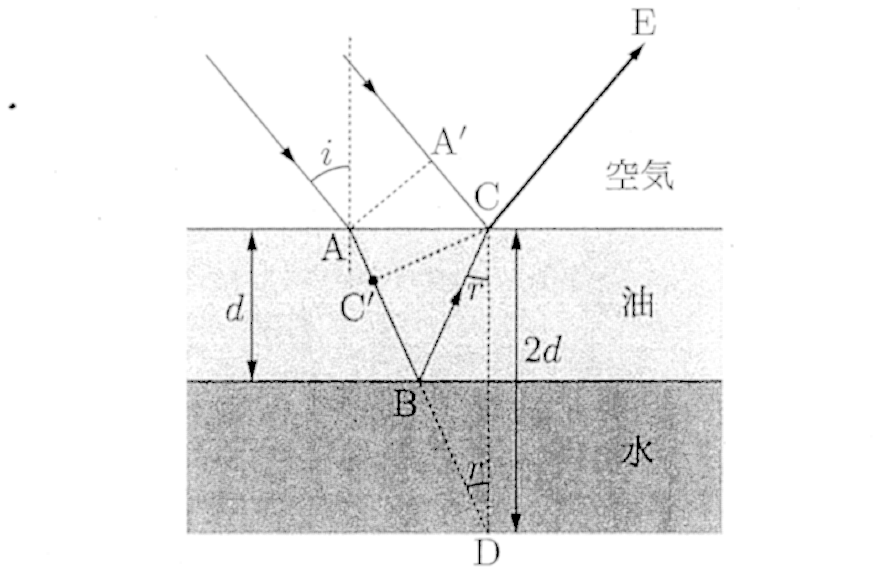
\includegraphics[keepaspectratio,width=62mm]{fig/n19_a58_oil.png}\end{center}
% 点Dが定義されずに出てきていたので，折り返しの点であることを明記した（2026-09-14）。
       ここで，$\mathrm{C}$点を油と水の境界面に対称に折り返した点が図の$\mathrm{D}$である．$\mathrm{C^\prime\sim B\sim C}$の部分の幾何学的距離は図の$\mathrm{C^\prime\sim B\sim D}$の長さと同じで，これは屈折角を$r$とすると
       \[2d\cos r\U{m}\]
       である．よって，この二つの光の光路差$\Delta$は，
       \[\Delta=2nd\cos r\U{m}\]
       ここで，$\mathrm{A}$点での屈折の法則より，
       \[\sin i=n\sin r\]
       が成立するので，$\sin r=\dfrac{\sin i}{n}$である．これより，
       \[\cos r=\sqrt{1-\sin^2 r}=\sqrt{1-\frac{\sin^2 i}{n^2}}\]
       であるからこれを代入して$r$を消すと，
       \[\Delta=2d\sqrt{n^2-\sin^2 i}\U{m}\Ans\]
\ko{2} この二つの光の経路において反射が起こるのは，下側の経路を回ってくる光の$\mathrm{B}$点での反射と，上側の経路をたどる光の$\mathrm{C}$点での反射の二つである．

       前者の$\mathrm{B}$点での反射については，油の屈折率$>$水の屈折率であるから，屈折率のより小さいものにぶつかって反射しているので，反射しても位相はずれない．

       後者の$\mathrm{C}$点での反射については，空気の屈折率$<$油の屈折率であるから，屈折率のより大きいものにぶつかって反射しているので，反射することによって位相が$\pi$ずれる．

       以上より，反射することによる位相のずれは全部で$\pi$となるので，光路差によってさらに$\pi$のずれが生じるとき，すなわち光路差が真空中1波長の整数倍＋半波長になっているときに$\mathrm{E}$方向への二つの光が強め合う．よって強め合うのは，
       \[2d\sqrt{n^2-\sin^2 i}=m\lambda+\frac{\lambda}{2}\]
       の条件が満たされるときである．これより，強め合う光の波長は，
       \[\lambda=\frac{4d}{2m+1}\sqrt{n^2-\sin^2 i}\U{m}\Ans\]
       \begin{bsHosoku}{参考}
       (2)の答えが表している波長をすべて列記すると，
       \[\frac{4d}{1}\sqrt{n^2-\sin^2 i},\ \frac{4d}{3}\sqrt{n^2-\sin^2 i},\]
       \[\frac{4d}{5}\sqrt{n^2-\sin^2 i},\ \frac{4d}{7}\sqrt{n^2-\sin^2 i},\ \cdots\]
       であり，これは整数値$m$を利用して
       \[\lambda=\frac{4d}{2m-1}\sqrt{n^2-\sin^2 i}\U{m}\]
       と書き表すこともでき，これでも正解である．本問の場合には，単に「整数値$m$」としか記されていないので，この答えでも上に列記したすべての波長を表せるので正解である．

       しかし，例えば問題文で「自然数$m$を用いて」と書かれていた場合，$\lambda=\dfrac{4d}{2m+1}\sqrt{n^2-\sin^2 i}\U{m}$の答えの式では上で列記した$\dfrac{4d}{1}\sqrt{n^2-\sin^2 i}\U{m}$の波長が含まれない（$m\geqq 1$であるため）ことになるため，間違いとなる．この場合には$\lambda=\dfrac{4d}{2m-1}\sqrt{n^2-\sin^2 i}\U{m}$と書けばすべての波長を表すことができる．

       問題文に与えられている文字が，整数値なのか，自然数（$\leftarrow$0を含んでいない）なのか，負でない整数値（$\leftarrow$0を含んでいる）なのかをしっかり読み取った上で，すべての波長を表せるような答えの書き方をしなければならない．また，より厳密には(2)のような場合でも$m$の値の変域をきちんと明示した方がよい（例えば$\lambda=\dfrac{4d}{2m+1}\sqrt{n^2-\sin^2 i}\U{m}$であれば$m\geqq 0$というように）．
       \end{bsHosoku}
\ko{3} 垂直に入射するときは$i=0^\circ$であること，また$d=5.0\times 10^{-7}\U{m}$であることに注意して各値を代入し，強め合いとなる波長を求めると，
       \[\lambda=\frac{3.0\times 10^{-6}}{2m+1}\U{m}\hspace{3mm}(m\geqq 0)\]
       である．この値が$380\U{nm}$〜$780\U{nm}$の範囲に入るのは$m=2$, 3の二つだけで，それぞれ
       \[\lambda=6.0\times 10^2\U{nm},\ 4.3\times 10^2\U{nm}\Ans\]
\ko{4} 同様に，$d=1.0\times 10^{-3}\U{m}$として整理すると，
       \[\lambda=\frac{6.0\times 10^{-3}}{2m+1}\U{m}\]
       であり，この値が$380\U{nm}$〜$780\U{nm}$の範囲に入るのは，
       \[380\times 10^{-9}\leqq\frac{6.0\times 10^{-3}}{2m+1}\leqq 780\times 10^{-9}\]
       を解いて，
       \[3846\leqq m\leqq 7894\]
       のとき．約4000種類もの様々な波長の光が強め合いの条件を満たし，これらが混ざり合う．$380\U{nm}$〜$780\U{nm}$の範囲のほとんどすべての光が混ざり合っているので，反射光は{\gtfamily 白色光に見える．}\hspace*{\fill}\Ans
\end{komon}

\Rank{C問題}
\MonN{59}{ゆがみのあるくさびガラス}\par\nopagebreak
\begin{sisin}
本問のようにガラスを平行移動させた場合の明線・暗線の移動を考えさせる問題では，{\gtfamily 同じ経路差を持つ点がどちらに移動するのか}を考えよ．例えば，ガラス$\mathrm{A}$を上方向に動かした場合は同じ空気厚を持つ点は左へ移動するので，明暗は左へ移動する．

また(3)では上から見た図と横から見た図を組み合わせて考えよう．
\end{sisin}
\KaiHead
\begin{komon}
% 旧版は(1)に図が無いのに「図の縦の矢印」と書き，「だけ異なる」の脱字があり，
% 設問が暗線間隔なのに明線間隔を答えていた。図を補い3点とも直した（2026-09-14）。
\ko{1} 隣り合う二つの暗線を考える．暗線の間隔も明線の間隔も等しいので，ここでは隣り合う二つの暗線位置の空気厚の差から求める．隣り合う暗線の間隔を$d\U{m}$とすると，この二つの位置の空気厚の差は次図の縦の矢印の長さであり，光路差の差はその2倍（往復分）の$2\times d\tan\theta\U{m}$である．
       \begin{center}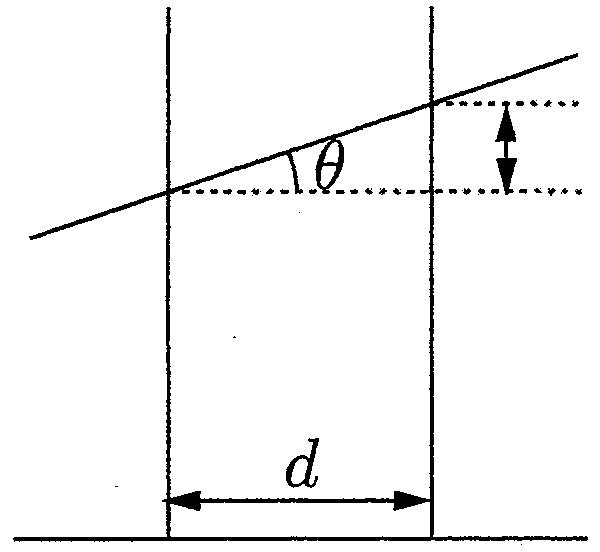
\includegraphics[keepaspectratio,width=34mm]{fig/n19_wedge_pitch.png}\end{center}
       一般に，隣り合う二つの暗線位置の光路差は$\lambda\U{m}$だけ異なるので，
       \[2\times d\tan\theta=\lambda\]
       が成立する．これを解いて，暗線の間隔は
       \[d=\frac{\lambda}{2\tan\theta}\fallingdotseq\frac{\lambda}{2\theta}\U{m}\Ans\]
\ko{2} 明線・暗線が右・左のどちらへ動くかは，同じ経路差を持つ点が右・左のどちらへ移動するかによって決まる．同じ空気厚を持つ点が右へ移動するためには$\mathrm{A}$板を下方向へ平行移動させればよい（次図参照．$\mathrm{A}$板を$\mathrm{A^\prime}$の位置に移動すると，太線で表される空気厚の位置は右へ移動するので，例えば左の太線のところで明線条件が満たされていたとき$\mathrm{A}$板を$\mathrm{A^\prime}$の位置に移動すると，その明線は右の太い点線の位置へと移動する）．
       \begin{center}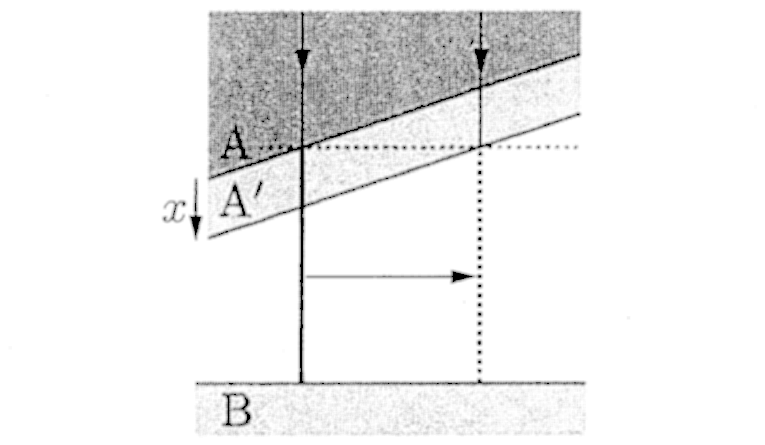
\includegraphics[keepaspectratio,width=54mm]{fig/n19_a59_move.png}\end{center}
       また，明線を右方向へ距離$d\U{m}$だけ移動させるためには，板$\mathrm{A}$を下方向へ距離
       \[x=d\tan\theta=\frac{\lambda}{2}\U{m}\]
       だけ動かせばよい．よって，縞模様を10本分だけ右方向へずらすためには，$\mathrm{A}$板を{\gtfamily 下方向へと距離}
       \[10x=5\lambda\U{m}\]
       {\gtfamily だけ移動させればよい．}\hspace*{\fill}\Ans
\ko{3} 暗線が2本分だけ右へずれた位置があるということは，右へずれている位置は暗線2本分だけ左の位置の空気厚しか持っていないということを意味する．これは$\mathrm{A}$板が次図のようにふくらんでいる場合でなければ起こらないので，$\mathrm{A}$板の下面は{\gtfamily ふくらんでいる．}\hspace*{\fill}\Ans
       \begin{center}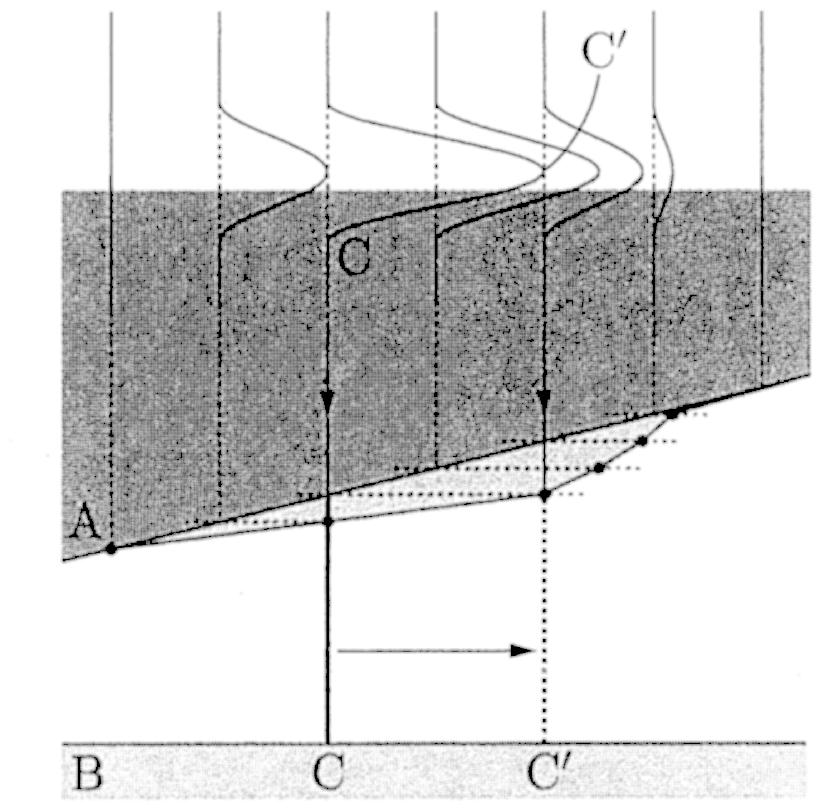
\includegraphics[keepaspectratio,width=58mm]{fig/n19_a59_bulge2.png}\end{center}
       この図において，上の図の$\mathrm{C}$の位置では下の図の$\mathrm{C}$の位置の太実線の空気厚を持っていて暗線条件が満たされている．同じ暗線条件がふくらみのある部分で満たされるのは$\mathrm{C^\prime}$の位置であるから，$\mathrm{C^\prime}$の位置での空気厚は$\mathrm{C}$点の空気厚と同じ太点線分である．同様に各々のずれについて考えていくと，ふくらみはこの図のように作図できる．

       よって，最大のふくらみを持つ点は図の$\mathrm{C^\prime}$の位置であり，次図を参照してそのふくらみを計算すると，
       \begin{center}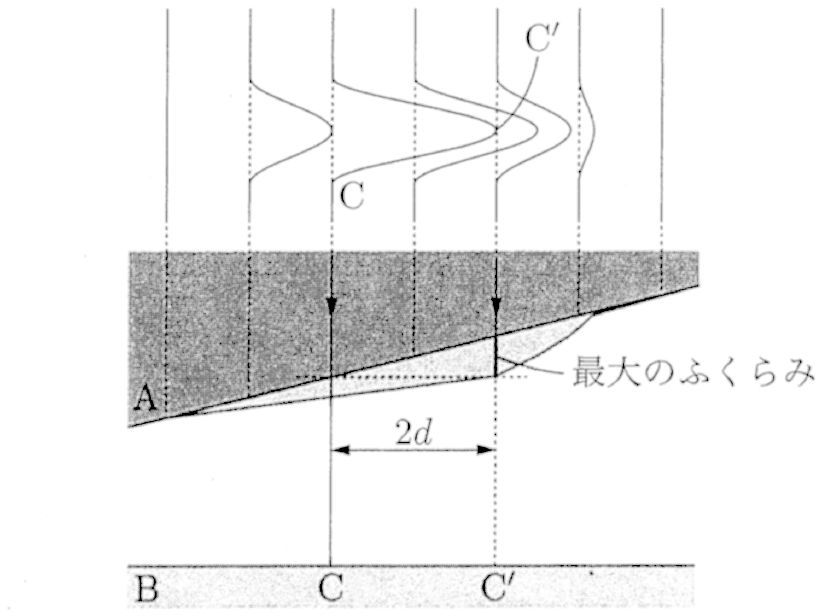
\includegraphics[keepaspectratio,width=58mm]{fig/n19_a59_bulge1.png}\end{center}
       \[(\text{最大のふくらみ})=2d\tan\theta=\lambda\U{m}\Ans\]
       となる．
\end{komon}

\MonN{60}{円形スリットによる干渉}\par\nopagebreak
\begin{sisin}
これも一見すると見たことのないタイプの難問のように見えるが，誘導に従っていけばたいした難問ではない．近似計算のみに注意して問題を解いていこう．
\end{sisin}
\KaiHead
\begin{komon}
\ko{1} 題意より，図2において
       \[\overline{\mathrm{S}_m\mathrm{F}}-\overline{\mathrm{S_0F}}=m\lambda\]
       が成立する，というのだから，これを$r_m$, $f$で表すと
       \[\sqrt{r_m^{\,2}+f^2}-f=m\lambda\]
       となる．ここで，$f\gg r_N\geqq r_m$であるから，
       \begin{align*}
       \sqrt{r_m^{\,2}+f^2}&=f\times\left\{1+\left(\frac{r_m}{f}\right)^2\right\}^{\frac{1}{2}}\\
       &\fallingdotseq f\times\left\{1+\frac{1}{2}\left(\frac{r_m}{f}\right)^2\right\}\\
       &=f+\frac{r_m^{\,2}}{2f}
       \end{align*}
       と近似できるので，
       \[\sqrt{r_m^{\,2}+f^2}-f=\frac{r_m^{\,2}}{2f}=m\lambda\]
       である．よってこれを解いて，
       \[r_m=\sqrt{2mf\lambda}\U{m}\Ans\]
\ko{2} 題意は，図3において
       \[\left(\overline{\mathrm{AS}_m}+\overline{\mathrm{S}_m\mathrm{B}}\right)-\left(\overline{\mathrm{AS_0}}+\overline{\mathrm{S_0B}}\right)=m\lambda\]
       が成立するということを意味する．これを$a$, $b$, $r_m$を用いて表すと，
       \[\overline{\mathrm{AS}_m}+\overline{\mathrm{S}_m\mathrm{B}}=\sqrt{a^2+r_m^{\,2}}+\sqrt{b^2+r_m^{\,2}}\]
       \[\overline{\mathrm{AS_0}}+\overline{\mathrm{S_0B}}=a+b\]
       であり，ここで$a$, $b\gg r_N>r_m$の関係を利用して近似を行うと，
       \begin{align*}
       &\overline{\mathrm{AS}_m}+\overline{\mathrm{S}_m\mathrm{B}}\\
       &\fallingdotseq a\left\{1+\frac{1}{2}\left(\frac{r_m}{a}\right)^2\right\}+b\left\{1+\frac{1}{2}\left(\frac{r_m}{b}\right)^2\right\}\\
       &=a+\frac{r_m^{\,2}}{2a}+b+\frac{r_m^{\,2}}{2b}
       \end{align*}
       であるから，
       \begin{align*}
       &\left(\overline{\mathrm{AS}_m}+\overline{\mathrm{S}_m\mathrm{B}}\right)-\left(\overline{\mathrm{AS_0}}+\overline{\mathrm{S_0B}}\right)\\
       &\fallingdotseq\frac{r_m^{\,2}}{2a}+\frac{r_m^{\,2}}{2b}
       \end{align*}
       となる．ここで(1)で求めた$r_m$を代入して整理すると，
       \[\frac{r_m^{\,2}}{2a}+\frac{r_m^{\,2}}{2b}=\frac{mf\lambda}{a}+\frac{mf\lambda}{b}\]
       となり，これが$=m\lambda$となるのだから，整理すると
       \[\frac{1}{a}+\frac{1}{b}=\frac{1}{f}\Ans\]
\ko{3} 水の中では波長が$\dfrac{\lambda}{n}\U{m}$になることに注意すると，題意は図4において
       \[\overline{\mathrm{S}_m\mathrm{F^\prime}}-\overline{\mathrm{S_0F^\prime}}=m\frac{\lambda}{n}\]
       が成立する，ということを意味する．これを$r_m$, $f^\prime$で表すと
       \[\sqrt{r_m^{\,2}+f^{\prime 2}}-f^\prime=m\frac{\lambda}{n}\]
       となる．ここで，$f^\prime\gg r_N>r_m$であるから，(1)と同様に
       \[\sqrt{r_m^{\,2}+f^{\prime 2}}\fallingdotseq f^\prime+\frac{r_m^{\,2}}{2f^\prime}\]
       と近似できるので，
       \[\sqrt{r_m^{\,2}+f^{\prime 2}}-f^\prime=\frac{r_m^{\,2}}{2f^\prime}=m\frac{\lambda}{n}\]
       である．これに(1)の答えの$r_m=\sqrt{2mf\lambda}\U{m}$を代入すると，
       \[\frac{2mf\lambda}{2f^\prime}=m\frac{\lambda}{n}\]
       となるので，これを整理して
       \[f^\prime=nf\U{m}\Ans\]
\end{komon}

\MonN{61}{マイケルソン干渉計}\par\nopagebreak
\begin{sisin}
テキストで扱ってきたヤングの実験，くさびガラス，平行薄膜，ニュートンリング，回折格子が主だった干渉の実験であるが，この他に有名な干渉の問題として，\MARU{1}マイケルソン干渉計，\MARU{2}単スリット干渉，といったものがある．これらは主に受験科で取り扱うが，このうち\MARU{1}のマイケルソン干渉計は今まで学んできた知識のみで簡単に解ける問題である．干渉する二つの光がたどる経路をはっきりさせてから光路差，および反射による位相のずれを考えて$\mathrm{D}$での強め合い・弱め合いを決めよう．

平面鏡$\mathrm{M_1}$を移動させると往復分だけ光路が増えるので，{\gtfamily 移動距離の2倍分だけ光路差が変化する}ことに注意．
\end{sisin}
\KaiHead
\begin{komon}
\ko{1} 光検出器$\mathrm{D}$に入射する光は，
       \[\MARU{1}:\mathrm{S\to H\to M_1\to H\to D}\ \text{と進む光}\]
       \[\MARU{2}:\mathrm{S\to H\to M_2\to H\to D}\ \text{と進む光}\]
       の二つが重なったものである．この二つの光の経路のうち，$\mathrm{S\to H}$の部分と$\mathrm{H\to D}$の部分は共通であるから，光路差は$\mathrm{H\to M_1\to H}$の部分と$\mathrm{H\to M_2\to H}$の部分との差分によって生じる．よって，二つの経路の光路差は，
       \begin{align*}
       &\left(\overline{\mathrm{OM_1}}+\overline{\mathrm{M_1O}}\right)-\left(\overline{\mathrm{OM_2}}+\overline{\mathrm{M_2O}}\right)\\
       &=2\times l_1-2\times l_2\U{m}
       \end{align*}
       である．\MARU{1}の経路では，最初の$\mathrm{H}$を通過する際には位相は変化せず（透過では位相は決してずれない），$\mathrm{M_1}$の反射で位相が$\pi$ずれ，戻ってきて$\mathrm{H}$で$\mathrm{D}$に向かって反射する際に位相が$\pi$ずれる．また\MARU{2}の経路では，最初に$\mathrm{H}$にぶつかって$\mathrm{M_2}$へ向けて反射する際に位相が$\pi$ずれ，続いて$\mathrm{M_2}$の反射で位相が$\pi$ずれ，戻ってきて$\mathrm{H}$を通過する際には位相はずれない．よってこれらを合わせると反射で位相は$2\pi-2\pi=0$とずれていないことになるので，$\mathrm{D}$で光が強め合う条件は，
       \[2\times l_1-2\times l_2=i\lambda\hspace{3mm}(\text{ただし}i\text{は整数値})\Ans\]
\ko{2} $\mathrm{M_1}$を遠ざけていくと，二つの光の経路\MARU{1}，\MARU{2}の光路差$\left(\overline{\mathrm{OM_1}}+\overline{\mathrm{M_1O}}\right)-\left(\overline{\mathrm{OM_2}}+\overline{\mathrm{M_2O}}\right)$は増加していくが，光路差が$\lambda\U{m}$ずつ増加するごとに再び強め合いの条件が満たされる．

       ここで，次図にあるように$\mathrm{M_1}$を遠ざけていくと往復分だけ光路差が増加するので，$\mathrm{M_1}$を距離$\dfrac{\lambda}{2}\U{m}$だけ動かすと光路差が$\lambda\U{m}$だけ増加する．
       \begin{center}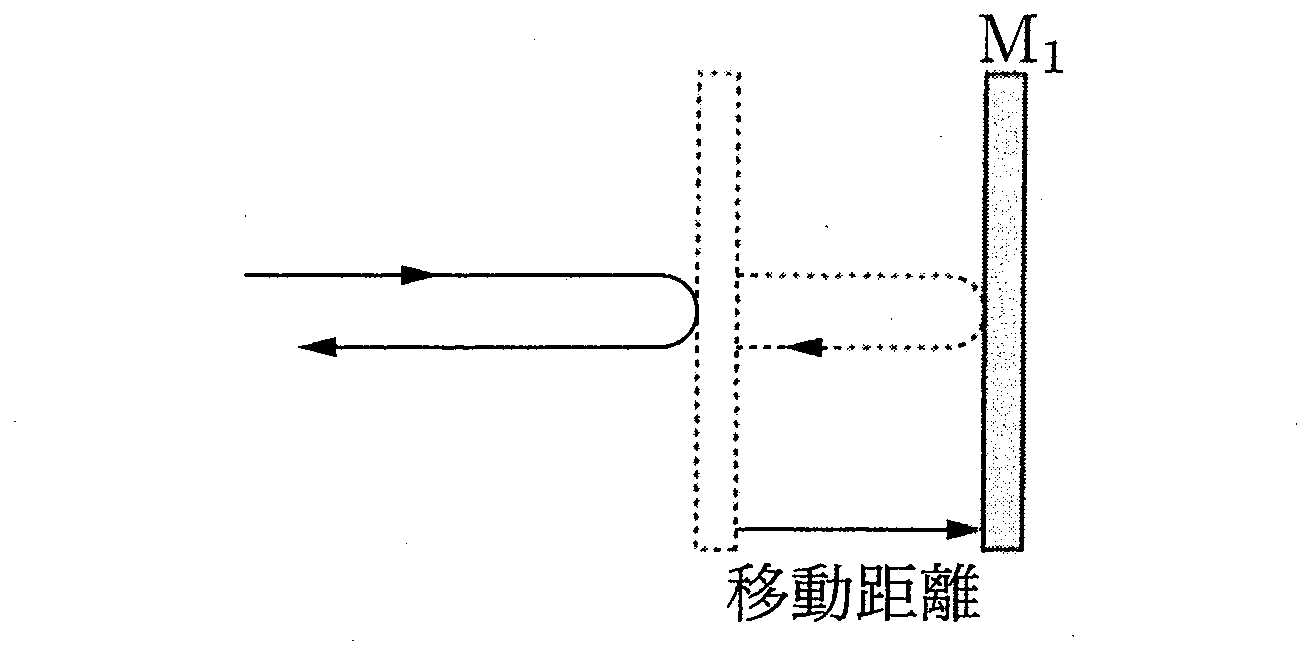
\includegraphics[keepaspectratio,width=54mm]{fig/n19_a61_move.png}\end{center}
       よって，反射鏡$\mathrm{M_1}$を距離$\dfrac{\lambda}{2}\U{m}$だけ動かすたびに再び強め合って明るくなるので，$m$回，明るくなるのを繰り返すためには
       \[\Delta x=m\frac{\lambda}{2}\U{m}\Ans\]
       だけ反射鏡$\mathrm{M_1}$を移動させればよい．
\end{komon}

\MonN{62}{反射光の干渉}\par\nopagebreak
\begin{sisin}
各平面部分からホイヘンスの原理に従って素元波が出て反射していき，それらが互いに干渉しあって強め合い・弱め合いを生じるため，必ずしも垂直に入射した光は垂直に反射していくだけではない（もちろん実際には，鉛直上向きに跳ね返る方向はすべての波長に対して強め合いとなるため光が最も強度的に強くなり，これを0次光と呼ぶ）．

斜めに光が跳ね返る方向を決めるためには，斜めに跳ね返ったときに光が強め合うための条件を求めればよく，これは今まで学んできた，経路差が一波長の整数倍となるか否かで判定ができる．これを考えていこう．
\end{sisin}
\KaiHead
\begin{komon}
\ko{1} 間隔$d\U{m}$を隔てた隣り合う平面部から反射した光との経路差は次図の太線部で与えられる．
       \begin{center}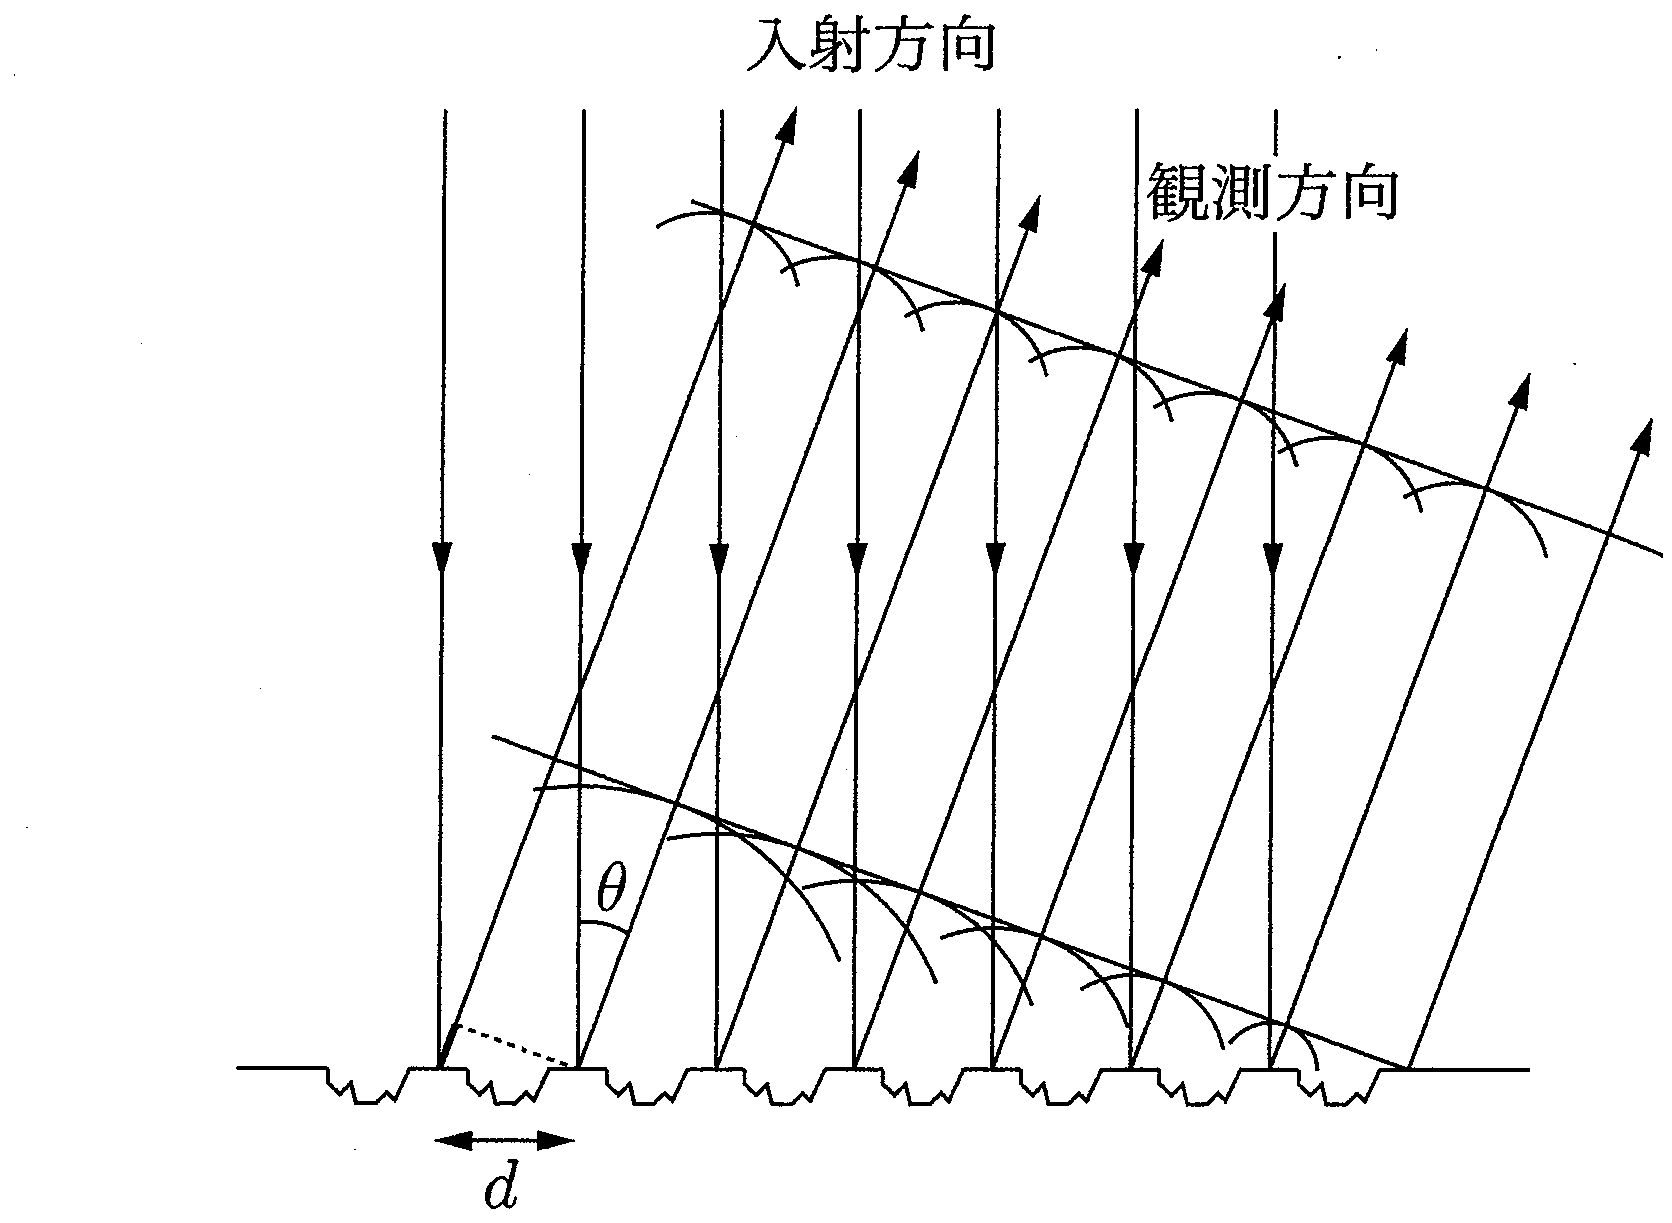
\includegraphics[keepaspectratio,width=58mm]{fig/n19_a62_path.png}\end{center}
       この経路差は長さ$d\sin\theta\U{m}$であり，これが
       \[d\sin\theta=m\lambda\]
       の条件を満たすとき，隣り合うすべての平面部から反射した光が強め合う．\hspace*{\fill}\Ans
\ko{2} $\theta=0^\circ$の場合にはすべての波長の光が強め合うので，これは最も強い反射であることは明らかである．光の強め合いが起こる角度$\theta_1$は，$m=1$で波長$400\U{nm}$の光に対しての強め合いが起こる角度であり，$\theta_2$は$m=1$で波長$700\U{nm}$の光に対しての強め合いが起こった直後である．よって，
       \[\sin\theta_1=\frac{1}{d}\times(400\times 10^{-9})\]
       \[\sin\theta_2=\frac{1}{d}\times(700\times 10^{-9})\]
       が成立する．溝の間隔$d\U{m}$は，
       \[d=\frac{1\times 10^{-2}}{6250}=1.6\times 10^{-6}\U{m}\]
       であるから，
       \[\sin\theta_1=0.25,\ \sin\theta_2=0.4375\]
       である．これらの値をグラフから読み取って，
       \[\theta_1\fallingdotseq 14^\circ,\ \theta_2\fallingdotseq 26^\circ\Ans\]
       である．
       \begin{chuu}
       与えられているグラフから角度を読み取るので，ある程度の誤差は許容される．$\pm 1^\circ$程度の食い違いなら正解としてよい．

       % 原本の注は「θ2≒27°の時点において」となっているが，(2)の答え（26°）と食い違うので合わせた．
       また厳密には，$\theta_2\fallingdotseq 26^\circ$の時点において，$m=2$，波長$400\U{nm}$の光の強め合いが始まっていないことを確認する必要がある．なぜなら，$m=1$の強め合いがすべての波長に対して終わるよりも前に$m=2$の強め合いが始まってしまうと，「角度$\theta_1$で強い光が見え始め，それは$\theta$の増加と共に色を変えながら角度$\theta_2$まで観測された」という題意の終点$\theta_2$は，$m=1$の強め合いの終わりの点（波長$700\U{nm}$の光に対する強め合いの点）とはならないからである．

       これを確かめると，$m=2$，波長$400\U{nm}$の光の強め合いが起こるのは，
       \[\sin\theta=\frac{1}{d}\times 2\times(400\times 10^{-9})=0.5\]
       であるから，これは明らかに先に求めた角度$\theta_2$よりも大きい．よって，確かに題意の強め合いの終点は$m=1$，波長$700\U{nm}$の光の強め合いの点であることが確認された．
       \end{chuu}
\ko{3} 光の波長が短いものから選んでいけばよいので，正解は
       \[\MARU{3}\Ans\]
       \begin{bsHosoku}{参考}
       光の色は波長と共に変化するが，その色の順番は虹の色の順番と同じである．これは覚えておかないと答えられないのでざっと覚えておこう．順番は，長波長側から，「赤，橙，黄，緑，青，藍，紫」（「せき・とう・おう・りょく・せい・らん・し」と暗記する）となっている．

       赤と紫のどちらが長波長，短波長に対応するかは次のようにして覚えよ．可視光領域を少しだけはずれた光を赤外光（もしくは赤外線），紫外光（もしくは紫外線）というが，これらは言葉からも分かるように，前者は「可視光の波長領域の赤の側から少しはみ出た光」，後者は「可視光の波長領域の紫の側から少しはみ出た光」を意味している．

       赤外線はコタツなどに利用されていることからも分かるように，エネルギー的に小さく，波長の長い電磁波で，熱をよく伝える．これに対して紫外線は海などの日焼けの話から分かるように，波長の短い電磁波である．よって，これらのことから紫側が短波長，赤側が長波長であることが分かる．
       \end{bsHosoku}
\end{komon}

\end{multicols}
